\documentclass[twoside,11pt]{article}

% Use JMLR style with preprint option
\usepackage[preprint]{jmlr2e}
\usepackage{amsmath}
\usepackage{bbm} 
% Additional packages (jmlr2e already includes: epsfig, amssymb, natbib, graphicx)
\usepackage{algorithm}
\usepackage{algorithmic}
\usepackage{subcaption}
\usepackage{xcolor}
\usepackage{tikz}
\usetikzlibrary{calc, arrows.meta, decorations.markings, patterns, shapes.geometric, positioning, 3d, decorations.pathmorphing}
\usepackage{array}
\usepackage{tabularx}
\usepackage{listings}
\lstset{basicstyle=\ttfamily, breaklines=true}
\usepackage{booktabs}

% Note: jmlr2e already defines theorem environments and proof
% Available: theorem, lemma, proposition, corollary, definition, example
% Manual definitions (no amsmath needed)
\newcommand{\softmax}{\operatorname{softmax}}
\newcommand{\KL}{\operatorname{KL}}
\newcommand{\Tr}{\operatorname{Tr}}
\begin{document}

% JMLR heading for preprint
\jmlrheading{}{2025}{}{}{}{}{Robert C. Dennis}

\title{Attention, Transformers, and Backpropagation are\\
Degenerate Limits of the Variational Free Energy Principle}

\author{\name Robert C. Dennis \email cdenn016@gmail.com \\
       \addr Independent Researcher\\
       \addr Leander, Texas 78641, USA}

\editor{TBD}

\maketitle

\ShortHeadings{Attention and Transformers as Free Energy}{Dennis}
\begin{abstract}
We present a unified gauge-theoretic formulation of attention and message communication in multi-agent Bayesian systems performing variational inference. Each agent is modeled as a smooth local section of an associated bundle with statistical manifold fiber over a noumenal base manifold $\mathcal{C}$. We demonstrate that in the isotropic, flat-bundle, Dirac-delta function limit (where all local frames coincide globally) the generalized attention weights reduce to the canonical transformer rule $\beta_{ij} \propto \softmax(Q_i K_j^\top)$ exactly and backpropagation training emerges as gradient descent on the free energy in the deterministic, flat-bundle limit—discarding the natural gradient structure that provides faster convergence. Starting from a generative model of inter-agent message exchange, we derive a generalized variational free-energy functional whose stationary points govern agent dynamics. In the absence of observations, this functional defines a gauge-symmetric vacuum theory in which all agents converge to identical beliefs modulo gauge orbit; introducing observations breaks this symmetry, leading to agent specialization. We validate our framework through simulations of $N=8$ agents with 9-dimensional Gaussian beliefs under SO(3) gauge transformations, demonstrating convergence to symmetric vacuum states and symmetry breaking under observation/training. We fully derive the equivalence to modern transformer architectures and backpropagation and show our framework suggests exponential speedup during training via natural gradient descent.
\end{abstract}

\noindent\textbf{Keywords:} gauge theory, free energy principle, transformer attention, variational inference, information geometry, natural gradient, symmetry breaking, multi-agent systems

\section{Introduction}

Recent advances in neuroscience and intelligent systems have independently converged on the idea that intelligent systems integrate perception, inference, and communication under the constraints of uncertainty \citep{bahdanau2014neural} \citep{amari1998natural} \citep{bronstein2021geometric} \citep{foerster2016learning}\citep{wooldridge2009introduction}. Friston’s Free Energy Principle (FEP) provides a general variational formulation of inference in cognitive systems\citep{friston2010free} \citep{parr2022active} \citep{friston2017graphical} \citep{ramstead2020variational}, whereas the attention mechanism in modern machine learning architectures defines a powerful (although empirically derived) rule for token prediction\citep{clark2019does} \citep{vaswani2017attention}. Despite their shared reliance on probabilistic inference and pairwise interaction, these two frameworks remain stubbornly separated. In particular, transformer attention lacks an underlying geometric or mathematical foundation and details on how and why modern machine learning architectures operate as well as they do remains obscure.

Many varieties of transformer and attention architectures have been proposed, implemented, and studied in recent years. \citep{fuchs2020se3}\citep{thomas2018tensor}.  Some architectures make use of bundle geometric frameworks but lack a first-principles foundation or connection to the FEP\citep{kondor2018generalization}\citep{finzi2020generalizing}\citep{bronstein2021geometric}.  Furthermore, attempts at curved space token embeddings have produced mixed results.\citep{bonnabel2013stochastic}\citep{absil2008optimization}

In this report we propose a unified, gauge-equivariant framework that connects these disparate yet similar domains. Our framework is based on a principled bundle geometry whereby each agent is modeled as a smooth local section of an associated bundle with statistical manifold fibers over a "noumenal" base manifold. Inter-agent communication arises naturally through a non-abelian gauge connection that defines parallel-transport operators between agents' local  gauge frames. Within this geometry, attention emerges as a gauge-aligned Kullback–Leibler (KL) term derived directly from the variational free energy of a coupled multi-agent generative model.

We then show that in the flat-bundle, isotropic, delta-function limit attention reduces to the standard transformer dot-product attention $QK^T$, thereby identifying transformer attention as a degenerate case of a broader geometric and statistical law of communication predicated upon the FEP.  We then show that hard, one-hot attention encoding is the zero-temperature limit of the FEP agent-agent coupling term and the large temperature limit leads to uniform encoding.  We demonstrate this by simulating a toy model of variational gradient descent under generalized free energy of multivariate Gaussian agents and by applying our alignment expression to a frozen transformer.  Finally, we describe the theory and numerical results that suggest that token encoding under data training (i.e. agent belief alignment) is a spontaneous symmetry breaking phenomenon of our gauge-theoretic framework.

Finally, we mathematically show that modern machine learning back propagation gradient descent and attention transformers the identically the Dirac flat limit of a more general gauge equivariant theory under natural gradient descent of the variational free energy functional.  Our results suggests that deep learning architectures can potentially achieve an exponential speedup during training by leveraging our gauge equivariant free energy formalism. 

\subsection{An intuitive simplification for non-geometers}
For interdisciplinary readers, it may be helpful to visualize each agent in this framework as a vector and a matrix field defined over a finite spatial region. 
Concretely, at every point $c$ in the base manifold, agent $i$ carries a mean vector $\mu_i(c)$ and a covariance matrix $\Sigma_i(c)$ representing, respectively, its local expected state and uncertainty. Together these form a smooth Gaussian field—the agent’s belief section of the statistical bundle. 

We will see that the agent's local gauge frame $\phi_i(c)$ may be intuitively interpreted as the agent's subjective frame of reference—its internal coordinate system through which beliefs and models are represented and compared. In this sense, $\phi_i(c)$ captures an agent’s “internal orientation” toward the world: it determines how external information is projected into the agent’s internal representational space. Gauge transformations $\phi_i(c) \to \phi_i(c) + \xi(c)$ thus correspond to changes in perspective that leave the underlying informational content invariant, much like shifts of viewpoint in perception that preserve the same world model. 

\begin{figure}[h]
\centering
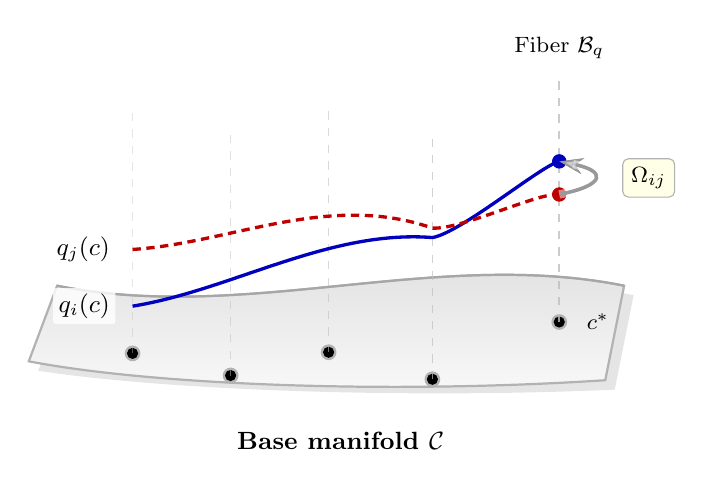
\begin{tikzpicture}[scale=1.2, every node/.style={font=\small}]
% requires \usetikzlibrary{calc, arrows.meta, decorations.markings, shadows}

% ------------------------------------------------------------------
% ENHANCED 3D BASE MANIFOLD with gradient and shadow
% ------------------------------------------------------------------
\path
  (0,0) coordinate (M1)
  (6,0) coordinate (M2)
  (5.8,-1.0) coordinate (M3)
  (-0.3,-0.8) coordinate (M4);

% Shadow layer
\filldraw[fill=black!10, draw=none]
  ($(M1)+(0.1,-0.1)$)
    .. controls (2.1,-0.5) and (4.1,0.3) .. ($(M2)+(0.1,-0.1)$)
    -- ($(M3)+(0.1,-0.1)$)
    .. controls (3.6,-1.2) and (1.1,-1.1) .. ($(M4)+(0.1,-0.1)$)
    -- cycle;

% Main surface with gradient
\shade[top color=gray!25, bottom color=gray!5, draw=gray!60, thick]
  (M1)
    .. controls (2,-0.4) and (4,0.4) .. (M2)
    -- (M3)
    .. controls (3.5,-1.15) and (1.0,-1.05) .. (M4)
    -- cycle;

% Surface outline for crispness
\draw[gray!70, thick]
  (M1)
    .. controls (2,-0.4) and (4,0.4) .. (M2);

\node[below, black, font=\small\bfseries] at (3,-1.45) {Base manifold $\mathcal{C}$};

% ------------------------------------------------------------------
% FIBER ANCHOR POINTS with improved positioning
% ------------------------------------------------------------------
\coordinate (C1) at ($(M4)!0.18!(M3)+(0,0.12)$);
\coordinate (C2) at ($(M4)!0.35!(M3)+(0,-0.08)$);
\coordinate (C3) at ($(M4)!0.52!(M3)+(0,0.20)$);
\coordinate (C4) at ($(M4)!0.70!(M3)+(0,-0.05)$);
\coordinate (C5) at ($(M4)!0.92!(M3)+(0,0.60)$);

% Anchor points with subtle glow
\foreach \c in {C1,C2,C3,C4,C5} {
  \filldraw[black!30] (\c) circle (2.2pt);
  \filldraw[black] (\c) circle (1.5pt);
}

% ------------------------------------------------------------------
% FIBERS with gradient opacity for depth
% ------------------------------------------------------------------
\foreach \c [count=\i] in {C1,C2,C3,C4,C5} {
  \pgfmathsetmacro{\opacity}{0.3 + \i*0.1}
  \draw[gray!50, dashed, line width=0.6pt, opacity=\opacity] 
    (\c) -- ++(0,2.6);
}

% Fiber label with better positioning
\node[above=3pt, black, font=\footnotesize] at ($(C5)+(0,2.6)$) {Fiber $\mathcal{B}_q$};

% ------------------------------------------------------------------
% SECTION CURVES with enhanced styling
% ------------------------------------------------------------------
% Section q_i (solid blue)
\draw[thick, blue!75!black, line width=1.2pt]
  ($(C1)+(0,0.5)$)
    .. controls ($(C2)+(0,0.9)$) and ($(C3)+(0,1.3)$)
    .. ($(C4)+(0,1.5)$)
    .. controls ($(C4)+(0.3,1.55)$) and ($(C5)+(-0.2,1.65)$)
    .. ($(C5)+(0,1.7)$);

% Section q_j (dashed red)
\draw[thick, red!75!black, densely dashed, line width=1.2pt]
  ($(C1)+(0,1.1)$)
    .. controls ($(C2)+(0,1.4)$) and ($(C3)+(0,1.7)$)
    .. ($(C4)+(0,1.6)$)
    .. controls ($(C4)+(0.3,1.58)$) and ($(C5)+(-0.2,1.38)$)
    .. ($(C5)+(0,1.35)$);

% Enhanced section labels with background
\node[left=6pt, black, fill=white, fill opacity=0.8, text opacity=1, 
      inner sep=2pt, rounded corners=1pt] 
  at ($(C1)+(0,0.5)$) {$q_i(c)$};
\node[left=6pt, black, fill=white, fill opacity=0.8, text opacity=1, 
      inner sep=2pt, rounded corners=1pt] 
  at ($(C1)+(0,1.1)$) {$q_j(c)$};

% Section endpoint markers
\filldraw[blue!75!black] ($(C5)+(0,1.7)$) circle (2pt);
\filldraw[red!75!black]  ($(C5)+(0,1.35)$) circle (2pt);

% Highlight the special point c*
\node[right=3pt, black, font=\footnotesize\itshape] 
  at ($(C5)+(0.1,0)$) {$c^*$};

% ------------------------------------------------------------------
% TRANSPORT OPERATOR with improved arrow
% ------------------------------------------------------------------
\draw[-{Stealth[length=3mm, width=2mm]}, very thick, black!80, 
      line width=1.3pt,
      postaction={draw, line width=3pt, white, opacity=0.5, -{Stealth[length=3mm, width=2mm]}}]
  ($(C5)+(0,1.35)$)
    .. controls ($(C5)+(0.5,1.45)$) and ($(C5)+(0.5,1.60)$)
    .. ($(C5)+(0,1.7)$);

% Transport label with background box
\node[right=5pt, black, fill=yellow!10, draw=black!30, 
      inner sep=3pt, rounded corners=2pt, font=\footnotesize\bfseries] 
  at ($(C5)+(0.52,1.525)$) {$\Omega_{ij}$};

\end{tikzpicture}
\caption{%
Visualization of agent sections $q_i(c)$ and $q_j(c)$ over an associated bundle. 
The shaded surface represents the base manifold $\mathcal{C}$, with vertical fibers $\mathcal{B}_q$ 
shown as dashed lines anchored at black points. 
At the reference point $c^*$ on the rightmost fiber, the transport operator $\Omega_{ij}(c^*)$ 
maps the red section value $q_j(c^*)$ into the blue section value $q_i(c^*)$, 
enabling frame alignment between agent representations.
}
\label{fig:bundle_sections_surface}
\end{figure}


\section{Methods}

We begin with a general geometric construction that naturally supports hierarchical emergence of meta-agents, scale interactions, and non-trivial holonomy of transport. The details of the most general geometry and framework can be found in the appendix and references \citep{nakahara2003geometry}\citep{kullback1951information} \citep{sternberg1994group}\citep{fulton1991representation}\citep{frankel2011geometry}\citep{baez1994gauge}.  Briefly, in this current report, we describe agents as modeled by a local section of an associated bundle to a principal $G$ fiber bundle. This framework enables a unified description of both intra-agent inference and inter-agent communication in terms of gauge frame transport and alignment.

\subsection{Code Availability}
The complete simulation suite that implements the gauge-theoretic variational inference framework described in this work is publicly available at 
\begin{itemize}
\item \href{https://github.com/cdenn016/epistemic-geometry}{https://github.com/cdenn016/epistemic-geometry}. 
\end{itemize}
The repository includes:
\begin{itemize}
  \item Core gradient modules (\lstinline|gradient_terms.py|, \lstinline|gradient_utils.py|)
  \item Natural gradient implementations (\lstinline|numerical_utils.py|)
  \item Gauge transport computations (\lstinline|transport_cache.py|, \lstinline|omega.py|)
  \item Multi-agent update (\lstinline|update_compute_all_gradients.py|, \lstinline|update_rules.py|)
  \item Stability monitoring and energy budget tracking (\lstinline|tests_and_stability|)
  \item Simulation driver and configuration (\lstinline|generalized_simulation.py|, \lstinline|config.py|)
  \item Diagnostic tools (\lstinline|diagnostics.py|, \lstinline|metrics_viz.py|)
\end{itemize}


All experiments reported in the results section can be reproduced using the provided configuration files and random number generator seeds documented in the repository. The codebase requires Python 3.9+ with NumPy, SciPy, and Joblib dependencies as specified in \texttt{requirements.txt}.

\subsection{Specializations for the Current Study}
Here we specify the simplifications adopted for the remainder of this work, which retain essential geometric structure while ensuring computational tractability and simplification.

\subsubsection{Matched Bundles}
In our general formulation agents are treated as pairs of sections of associated bundles $\mathcal{B}_q$ and $\mathcal{B}_p$ of beliefs and models.  Here we simplify by implementing

\begin{equation}
\mathcal{B}_q = \mathcal{B}_p =: \mathcal{B}, \qquad \rho_q = \rho_p =: \rho.
\end{equation}

This gives $\mathcal{E}_q = \mathcal{E}_p =: \mathcal{E}$, and the bundle morphisms become:

\begin{equation}
\Phi = \tilde{\Phi} = \text{id}_{\mathcal{E}}.
\end{equation}

Each agent then reduces to a single section $\sigma^i: \mathcal{U}_i \to \mathcal{E}$, with belief/prior distinction maintained through local fiber coordinates.

\subsubsection{Gaussian Fiber and SO(3) Gauge Group}
Next, we restrict to the exponential family of multi-variate Gaussian distributions with $G=SO(3)$.  That is,

\begin{itemize}
  \item Fiber: $\mathcal{B} = \{(\mu, \Sigma) : \mu \in \mathbb{R}^3, \Sigma \in \mathbb{R}^{3 \times 3}, \Sigma \succ 0\}$ (Gaussian manifold)
  \item Group: $G = SO(3)$ with representation:\\
\\
\begin{equation}
\rho(\Omega) \cdot (\mu, \Sigma) = (\Omega\mu, \Omega\Sigma\Omega^\top)
\end{equation}
\end{itemize}

The Gaussian manifold has constant negative curvature under the Fisher-Rao metric. The group $SO(3)$ has constant positive curvature and non-commutative composition.  These choices are motivated by computational flexibility while maintain a degree of geometric generality.  In particular, $SO(3)$ and its representation theory is well studied and present in a variety of fields.  However, our results can be directly extended to $SO(N)$ or even $SU(N)$ in the standard way \citep{nakahara2003geometry}\citep{hall2015lie}.

\subsubsection{Gauge Group and Representations}
Let us now consider the representation theory of $G = SO(3)$, which acts on the fibers via its representations:

\begin{equation}
\rho_q: SO(3) \to \mathrm{GL}(d_q), 
\qquad
\rho_p: SO(3) \to \mathrm{GL}(d_p).
\label{eq:representations}
\end{equation}

In full generality these representations may be reducible or irreducible thereby allowing even or odd dimensions to be studied.  For example, a token dimension of $768$ could be broken into the appropriate number of irreps (see below) necessary for an even dimension action \citep{hall2015lie}

For $\Omega \in SO(3)$, the gauge action on a Gaussian state is:

\begin{equation}
\boxed{
\begin{aligned}
\rho_q(\Omega) \cdot (\mu_q, \Sigma_q) 
&= \big(\rho_q(\Omega)\,\mu_q,\; 
\rho_q(\Omega)\,\Sigma_q\,\rho_q(\Omega)^\top\big),\\
\rho_p(\Omega) \cdot (\mu_p, \Sigma_p) 
&= \big(\rho_p(\Omega)\,\mu_p,\; 
\rho_p(\Omega)\,\Sigma_p\,\rho_p(\Omega)^\top\big).
\end{aligned}
}
\label{eq:gauge_action_gaussians}
\end{equation}

\subsubsection{Representation Structure}
The dimensions $d_q, d_p$ are not constrained to be 1, 3, 5, 7, $\ldots$ (irrep dimensions of $SO(3)$). Instead we may have $\rho_q, \rho_p$ as reducible representations built from direct sums of the irreps:

\begin{equation}
\rho_q \cong \bigoplus_{k} n_k \cdot \ell_k,
\quad
d_q = \sum_{k} n_k (2\ell_k + 1),
\label{eq:reducible_decomposition}
\end{equation}

where $\ell_k \in \{0, 1, 2, \ldots\}$ labels spin, $n_k \in \mathbb{N}$ is multiplicity, and irrep $\ell_k$ has dimension $2\ell_k + 1$.

Example: A $d_q = 768$ dimensional embedding with gauge group $G = SO(3)$ could decompose as:

\begin{equation}
\rho_q \cong 109 \cdot \ell_0 \oplus 49 \cdot \ell_1 \oplus 32 \cdot \ell_2 \oplus \ldots
\end{equation}

(109 scalars + 49 vectors + 32 rank-2 tensors + $\ldots$), where the $SO(3)$ gauge group acts on this high-dimensional space via the representation $\rho_q: SO(3) \to GL(768)$.

In the simulations we perform (see discussion) we used $d_q = d_p = 9$ with the irreducible spin-$4$ representation:

\begin{equation}
\rho_q = \rho_p = \ell_4, 
\quad
\text{(irrep, dimension $2 \cdot 4 + 1 = 9$)}.
\label{eq:simulation_irrep}
\end{equation}

\subsubsection{Gauge structure}
The gauge structure of our framework is built via the following:

\begin{itemize}
  \item Gauge group: $G = SO(3)$ (compact, 3 generators)
  \item Frame fields: $\phi_i(c) \in \mathfrak{so}(3)$ vary spatially
  \item Transport: $\Omega_{ij}(c) = e^{\phi_i(c)}e^{-\phi_j(c)} \in SO(3)$
  \item Action on fiber: $\rho(\Omega_{ij}) \in GL(d_K)$
\end{itemize}

In the transformer limit we will show that the gauge group becomes trivial:

\begin{equation}
G = SO(3) \to \{e\} \quad \text{(identity element only)}
\end{equation}

Therefore all gauge frames collapse to a single global shared space. I.e.

\begin{equation}
\phi_i(c) = \zeta =\text{const} \in \mathfrak{so}(3) \quad \forall i, c
\end{equation}

This then makes gauge transport trivial:

\begin{equation}
\Omega_{ij}(c) = \exp[\zeta] \exp[-\zeta] = \mathbb{I} \quad \forall i,j,c
\end{equation}

and the representation acts as the identity:

\begin{equation}
\rho(e) \cdot \mu_j = \mu_j 
\end{equation}

Therefore in this limit we have the following simplifications which lead to the transformer architecture from a more general and rich geometry:

\begin{itemize}
  \item Vanishing Induced Connection: $A_\mu = -\partial_\mu \phi_i = 0$
  \item Vanishing Curvature: $F_{\mu\nu} = 0$ (flat bundle)
  \item A single global coordinate system
  \item The gauge-aligned KL reduces to standard KL
\end{itemize}

\subsubsection{Role of learned projections $W_Q, W_K$}
In the trivial gauge limit, the query/key projections are not gauge transformations but rather are learned linear maps used to extract features.

$$
Q_i = W_Q^T \mu_i \in \mathbb{R}^{d_k},
$$

$$
K_j = W_K^T \mu_j \in \mathbb{R}^{d_k}
$$

These project from the full embedding space $\mathbb{R}^d$ (where $d$ can be arbitrarily large) to a lower-dimensional attention subspace $\mathbb{R}^{d_k}$ where similarity is computed in the standard way:

\begin{equation}
\alpha_{ij} = \text{softmax}_j\left(\frac{Q_i K_j^\top}{\sqrt{d_k}}\right)
\end{equation}

The following table summarizes the transformer limit:
\begin{table}[h]
\centering
\renewcommand{\arraystretch}{1.2}
\setlength{\tabcolsep}{6pt}
\begin{tabularx}{\textwidth}{lXX}
\hline
\textbf{Property} &
\textbf{Gauge Theory (SO(3))} &
\textbf{Transformer (trivial gauge)} \\
\hline
Gauge group $G$ &
$SO(3)$ (non-trivial) &
$\{e\}$ (trivial) \\
Frame field $\phi_i(c)$ &
Varies spatially &
$\phi_i = 0$ everywhere \\
Transport $\Omega_{ij}$ &
$e^{\phi_i} e^{-\phi_j} \neq \mathbb{I}$ &
$\mathbb{I}$ \\
Connection $A_\mu$ &
$-\partial_\mu \phi_i \neq 0$ &
$0$ \\
Curvature $F_{\mu\nu}$ &
Can be $\neq 0$ &
$0$ (flat) \\
KL coupling &
$D_{\text{KL}}[q_i \,\|\, \Omega_{ij} q_j]$ &
$D_{\text{KL}}[q_i \,\|\, q_j]$ \\
$W_Q, W_K$ role &
N/A (no projections) &
Feature extractors in flat space \\
Embedding dimension &
Any &
Any \\
\hline
\end{tabularx}
\caption{Comparison between the full gauge-theoretic formulation and the transformer limit.}
\label{tab:gauge_vs_transformer}
\end{table}



\subsubsection{Flat Base Manifold}
\begin{equation}
\mathcal{C} = \mathbb{R}^2 \quad \text{(Euclidean)}, 
\end{equation}

We consider the case of a flat base manifold (for simplicity and due to limited computational resources). Agents occupy finite support regions $\mathcal{U}_i$ as open subsets of $\mathbb{R}^2$ (where we invoke periodic boundary conditions in simulations).

\subsubsection{Local Gauge Frames}
Each agent $i$ has a gauge frame field $\phi_i: \mathcal{U}_i \to \mathfrak{so}(3)$ which may vary spatially. This induces a local connection:

\begin{equation}
A^{(i)}_\mu(c) = -\partial_\mu \phi_i(c) + \mathcal{O}(\phi_i^2),
\end{equation}

with field strength:

\begin{equation}
F^{(i)}_{\mu\nu}(c) = \partial_\mu A^{(i)}_\nu - \partial_\nu A^{(i)}_\mu + [A^{(i)}_\mu, A^{(i)}_\nu].
\end{equation}

In our simulations:

\begin{enumerate}
  \item Frames are smooth and slowly varying: $\|\partial_\mu \phi_i\| \ll 1$, so that $F^{(i)}_{\mu\nu} \approx 0$ locally
  \item We compute inter-agent transport pointwise (within the same fiber) using the Baker-Campbell-Hausdorff (BCH) formula:\\
\\
\begin{equation}
\Omega_{ij}(c) = e^{\phi_i(c)}e^{-\phi_j(c)}
\end{equation}
\end{enumerate}

This effectively treats gauge transport as local frame rotations without considering holonomy or global topology, which shall be saved for future study.

\subsubsection{Intra-Scale Transport Only}
We restrict to intra-scale transport operators $\Omega_{ij}: \Gamma(\mathcal{B}) \to \Gamma(\mathcal{B})$ between agents at the same hierarchical level. Cross-scale morphisms $\Lambda^s_{s'}$ and meta-agent emergence are deferred to future work with promising preliminary results.

\subsubsection{Gauge-Aligned Divergence}
With these assumptions, the gauge-aligned KL divergence between agents is (see appendix):

\begin{equation}
D_{\text{KL}}\left[q_i(c) \,\big\|\, \Omega_{ij}(c) q_j(c)\right],
\end{equation}

where for Gaussian beliefs:

\begin{equation}
\Omega_{ij}(c) \cdot (\mu_j, \Sigma_j) = \left(\Omega_{ij}(c)\mu_j, \, \Omega_{ij}(c)\Sigma_j\Omega_{ij}(c)^\top\right).
\end{equation}

This divergence forms the basis of our attention mechanism.


\begin{table}[h]
\centering
\renewcommand{\arraystretch}{1.15}
\setlength{\tabcolsep}{6pt}
\begin{tabularx}{\textwidth}{l>{\raggedright\arraybackslash}Xl}
\hline
\textbf{Symbol} & \textbf{Description} & \textbf{Type/Dimension} \\
\hline
\multicolumn{3}{l}{\textit{Fiber Bundle Structure}} \\
$\mathcal{M}$ & Base manifold (spatial domain) & Manifold \\
$Q_i$ & Belief fiber at agent $i$ & $\mathbb{R}^{K_q}$ \\
$P_i$ & Model fiber at agent $i$ & $\mathbb{R}^{K_p}$ \\
$G$ & Gauge group & $\mathrm{SO}(K)$ \\
$\mathfrak{g}$ & Lie algebra of $G$ & $\mathfrak{so}(K)$ \\
\\
\multicolumn{3}{l}{\textit{Gauge Fields and Connections}} \\
$\Omega^q_{ij}$ & Connection $Q_j \to Q_i$ & $\mathrm{SO}(K_q)$ \\
$\Omega^p_{ij}$ & Connection $P_j \to P_i$ & $\mathrm{SO}(K_p)$ \\
$\phi_i$ & Gauge parameter (belief frame) & $\mathfrak{g}\!\cong\!\mathbb{R}^3$ \\
$\tilde{\phi}_i$ & Gauge parameter (model frame) & $\mathfrak{g}\!\cong\!\mathbb{R}^3$ \\
$A_\mu(x)$ & Gauge connection field & $\mathfrak{g}$-valued 1-form \\
\\
\multicolumn{3}{l}{\textit{Bundle Morphisms}} \\
$\Phi_i$ & Morphism $Q_i \to P_i$ & $\mathbb{R}^{K_p\times K_q}$ \\
$\tilde{\Phi}_i$ & Morphism $P_i \to Q_i$ & $\mathbb{R}^{K_q\times K_p}$ \\
\\
\multicolumn{3}{l}{\textit{Statistical Parameters}} \\
$q_i(k_i)$ & Belief distribution & $\mathcal{N}(\mu_{q,i},\Sigma_{q,i})$ \\
$p_i(k_i)$ & Model distribution & $\mathcal{N}(\mu_{p,i},\Sigma_{p,i})$ \\
$\mu_{q,i},\mu_{p,i}$ & Mean vectors & $\mathbb{R}^{K_q},\mathbb{R}^{K_p}$ \\
$\Sigma_{q,i},\Sigma_{p,i}$ & Covariance matrices & $\mathbb{R}^{K\times K},\succ0$ \\
\\
\multicolumn{3}{l}{\textit{Attention and Coupling}} \\
$\beta_{ij}$ & Attention weight $j\!\to\!i$ & $[0,1]$ \\
$\tau$ & Attention temperature & $\mathbb{R}_+$ \\
$\alpha$ & Self-consistency strength & $\mathbb{R}_+$ \\
$D_{\mathrm{KL}}$ & Kullback–Leibler divergence & $\mathbb{R}_+\cup\{0\}$ \\
\hline
\end{tabularx}
\caption{Principal notation used throughout this paper.}
\label{tab:notation}
\end{table}



The full geometric framework enables exploration of:

\begin{itemize}
  \item Path-dependent parallel transport and holonomy effects
  \item Non-flat gauge connections with epistemic monopoles
  \item Curved base manifolds (hyperbolic/spherical latent spaces)
  \item Heterogeneous fiber structures ($\mathcal{B}_q \neq \mathcal{B}_p$)
  \item Cross-scale dynamics and meta-agent emergence
  \item Curvature-induced phase transitions in multi-agent\\
systems
  \item Pullback geometries via agent sections from informational fibers to the base manifold ("It from Bit", "qualia, etc")
\end{itemize}

\subsubsection{Rationale for Simplification}
These simplifications allow us to establish foundational results and demonstrate that transformer attention emerges from this gauge-theoretic free energy minimization geometry. Such simplifications further allow us to work within a single well-understood statistical manifold (Gaussian) and gauge group with known analytic properties and non-trivial curvatures\citep{amari2016information}.

For the present study, the matched bundle case ($\Phi = \text{id}$, $\mathcal{B}_q = \mathcal{B}_p$) suffices to establish the core theoretical result: transformer attention is the flat, isotropic, Dirac delta-function limit of gauge-covariant variational free energy minimization in multi-agent Bayesian systems. Furthermore data training and/or observations break the vacuum theory symmetry.

\section{Derivation of Generalized Variational Free Energy from a Normalized Generative Model}
We derive the generalized variational free energy we will utilize from general first principles, showing that both belief alignment (weighted by $\beta_{ij}$) and model alignment (weighted by $\gamma_{ij}$) emerge naturally from a single normalized generative prior with auxiliary agreement variables. This construction justifies the KL-based coupling terms as consequences of gauge-transported Gaussian consistency constraints. In what follows we shall assume all probability distributions are defined at a specific base manifold point $c = c^*$ unless otherwise noted.  We will label the fiber's latent coordinates as $k_i \in \mathcal{B}$ in order to define the necessary integrals

\subsection{Setup}
\subsubsection{Latent Variables and Fiber Geometry}
Each agent $i$ maintains two distinct latent variables living in separate fiber bundles:

\begin{equation}
k_i \in \mathbb{R}^{d_q} \quad \text{(belief latent in $\mathcal{E}_q$)}, 
\qquad
m_i \in \mathbb{R}^{d_p} \quad \text{(model latent in $\mathcal{E}_p$)}.
\label{eq:dual_latents}
\end{equation}

The full state of agent $i$ at base manifold point $c^*$is a Gaussian distribution over each latent:

\begin{equation}
\begin{aligned}
q_i(k_i) &= \mathcal{N}(k_i\,;\mu_{q,i},\,\Sigma_{q,i}), 
\quad \mu_{q,i} \in \mathbb{R}^{d_q},\; 
\Sigma_{q,i} \in \mathbb{R}^{d_q \times d_q}, \; \Sigma_{q,i} \succ 0,\\
s_i(m_i) &= \mathcal{N}(m_i\,;\mu_{p,i},\,\Sigma_{p,i}), 
\quad \mu_{p,i} \in \mathbb{R}^{d_p},\; 
\Sigma_{p,i} \in \mathbb{R}^{d_p \times d_p}, \; \Sigma_{p,i} \succ 0.
\end{aligned}
\label{eq:gaussian_states}
\end{equation}

Thus, the fiber at each agent's location $c \in \mathcal{C}$ is the product statistical manifold:

\begin{equation}
\mathcal{B}(c) = \mathcal{B}_q \times \mathcal{B}_p,
\label{eq:fiber_product}
\end{equation}

where

\begin{equation}
\begin{aligned}
\mathcal{B}_q &= \left\{
(\mu_q, \Sigma_q) : 
\mu_q \in \mathbb{R}^{d_q}, \;
\Sigma_q \in \mathbb{R}^{d_q \times d_q}, \;
\Sigma_q \succ 0
\right\},\\
\mathcal{B}_p &= \left\{
(\mu_p, \Sigma_p) : 
\mu_p \in \mathbb{R}^{d_p}, \;
\Sigma_p \in \mathbb{R}^{d_p \times d_p}, \;
\Sigma_p \succ 0
\right\}.
\end{aligned}
\label{eq:statistical_manifolds}
\end{equation}

\subsection{Base Priors}
Each latent has an independent Gaussian base prior encoding agent-specific inductive biases:

\begin{equation}
p_i(k_i) = \mathcal{N}(k_i\,; \mu_{0,i}^{(q)}, \Sigma_{0,i}^{(q)}), 
\qquad
r_i(m_i) = \mathcal{N}(m_i\,; \mu_{0,i}^{(p)}, \Sigma_{0,i}^{(p)}).
\label{eq:base_priors}
\end{equation}

These priors are \textbf{local}—they live in each agent's own gauge frame and need not be related across agents until transported via $\Omega_{ij}$.

\subsubsection{Auxiliary Agreement Variables}
To enforce consistency between agents after gauge transport, we introduce an auxiliary "agreement" variable for each ordered pair $(i,j)$:

\begin{equation}
z_{ij} \in \mathbb{R}^{d_q} \quad \text{(belief agreement)}, 
\qquad
w_{ij} \in \mathbb{R}^{d_p} \quad \text{(model agreement)}.
\label{eq:agreement_vars}
\end{equation}

\begin{itemize}
  \item $z_{ij}$: "What agent $i$ believes agent $j$'s belief looks like, after transporting $j$'s belief into $i$'s gauge frame"
  \item $w_{ij}$: "What agent $i$ believes agent $j$'s generative model looks like, after gauge transport"
\end{itemize}

These will be latent mediators that will be integrated out, leaving an effective pairwise coupling between $k_i, k_j$ and $m_i, m_j$.

Agreement variables allow us to construct a normalized joint generative model whose marginal over latents $\{k_i, m_i\}$ yield the desired gauge covariant pair potentials. This is in contrast to un-normalized Markov random fields, where potentials are imposed by fiat.

\subsection{Normalized Joint Generative Model}
We define the Gaussian couplings and enforce that each agreement variable $z_{ij}$,$w_{ij}$ simultaneously matches:

\begin{enumerate}
  \item Agent $i$'s own latent $k_i$, $m_i$
  \item Agent $j$'s latent $k_j$, $m_j$ after gauge transport into agent $i$'s frame
\end{enumerate}

The auxiliary variable $z_{ij}$ is drawn from the product of Gaussians:

\begin{equation}
p(z_{ij} \mid k_i, k_j) \propto 
\mathcal{N}(z_{ij}; k_i, \Lambda_{ij}^{-1}) \cdot 
\mathcal{N}(z_{ij}; \Omega_{ij}k_j, \Lambda_{ij}^{-1})
\label{eq:belief_coupling_product}
\end{equation}

and similarly for model alignment:

\begin{equation}
p(w_{ij} \mid m_i, m_j) \propto 
\mathcal{N}(w_{ij}; m_i, \Gamma_{ij}^{-1}) \cdot 
\mathcal{N}(w_{ij}; \tilde{\Omega}_{ij}m_j, \Gamma_{ij}^{-1})
\label{eq:model_coupling_product}
\end{equation}

where:

\begin{itemize}
  \item $\Lambda_{ij} \in \mathbb{R}^{d_q \times d_q}$, $\Lambda_{ij} \succ 0$: Belief alignment precision
  \item $\Gamma_{ij} \in \mathbb{R}^{d_p \times d_p}$, $\Gamma_{ij} \succ 0$: Model alignment precision
  \item $\Omega_{ij} \in SO(3)$: Gauge transport from agent $j$'s frame to agent $i$'s frame (belief channel)
  \item $\tilde{\Omega}_{ij} \in SO(3)$: Gauge transport from agent $j$'s frame to agent $i$'s frame (model channel)
\end{itemize}

\subsubsection{Gauge Transport as Frame Rotation}
The gauge transport operators $\Omega_{ij}, \tilde{\Omega}_{ij}$ are not parallel transport along a connection in the usual sense (which would be path-dependent). Instead, they are pointwise gauge frame rotations:

\begin{equation}
\Omega_{ij}(c) = e^{\phi_i(c)} \cdot e^{-\phi_j(c)} \in SO(3),
\label{eq:gauge_frame_rotation}
\end{equation}

where $\phi_i: \mathcal{U}_i \to \mathfrak{so}(3)$ is agent $i$'s gauge frame field (a local section of the Lie algebra bundle).

These act on the latent variables as

\begin{equation}
\begin{aligned}
\Omega_{ij} k_j 
&:= \rho_q(\Omega_{ij}) \, k_j 
\in \mathbb{R}^{d_q},\\
\tilde{\Omega}_{ij} m_j 
&:= \rho_p(\tilde{\Omega}_{ij}) \, m_j 
\in \mathbb{R}^{d_p}.
\end{aligned}
\label{eq:gauge_action_on_vectors}
\end{equation}

Later we invoke the transformer limit and take $\rho_q(\Omega_{ij}) = \mathbb{I}$, so $\Omega_{ij} k_j = k_j$ (trivial transport).

\subsubsection{Full Joint Distribution}
The joint generative model over all latents and auxiliary variables is:

\begin{equation}
\boxed{
\begin{aligned}
p&(\{k_i\},\{m_i\},\{z_{ij}\},\{w_{ij}\})\\
&=\left[\prod_i p_i(k_i)\,r_i(m_i)\right]\\
&\quad\times
\left[\prod_{i,j}
\mathcal{N}(z_{ij}\,;k_i,\Lambda_{ij}^{-1})
\,\mathcal{N}(z_{ij}\,;\Omega_{ij}k_j,\Lambda_{ij}^{-1})\right]\\
&\quad\times
\left[\prod_{i,j}
\mathcal{N}(w_{ij}\,;m_i,\Gamma_{ij}^{-1})
\,\mathcal{N}(w_{ij}\,;\tilde{\Omega}_{ij}m_j,\Gamma_{ij}^{-1})\right].
\end{aligned}
}
\label{eq:joint_distribution}
\end{equation}

The joint distribution \eqref{eq:joint_distribution} is properly normalized:

\begin{equation}
\int \prod_i dk_i\,dm_i \prod_{i,j} dz_{ij}\,dw_{ij} \;
p(\{k_i\},\{m_i\},\{z_{ij}\},\{w_{ij}\}) = 1.
\label{eq:normalization_check}
\end{equation}

\begin{proof}
Each factor is a normalized Gaussian:
\begin{itemize}
  \item Base priors $p_i(k_i)$, $r_i(m_i)$: normalized by definition
  \item Agreement couplings: products of Gaussians with identical precision, which yield normalized Gaussians after integrating over $z_{ij}, w_{ij}$
\end{itemize}

Since \eqref{eq:joint_distribution} is a product of normalized densities over disjoint variable sets (with auxiliary variables mediating), it is normalized.
\end{proof}

This is in contrast to unnormalized Markov random fields of the form $p(\{k_i\}) \propto \exp[-\sum_{ij} \psi_{ij}(k_i, k_j)]$, where the partition function $Z$ is intractable\citep{amari1985differential}. Our construction guarantees $Z = 1$ by design.
\subsection{Variational Free Energy}
We now form the variational free energy under a mean-field posterior approximation. Assume a factorized posterior
\begin{equation}
q(\{k_i\},\{m_i\})=\prod_i q_i(k_i)\,s_i(m_i),
\label{eq:mean_field_posterior}
\end{equation}
with Gaussian factors
\begin{equation}
q_i(k_i)=\mathcal{N}(k_i;\mu_{q,i},\Sigma_{q,i}),
\qquad
s_i(m_i)=\mathcal{N}(m_i;\mu_{p,i},\Sigma_{p,i}).
\label{eq:gaussian_factors}
\end{equation}
The variational free energy is defined as
\begin{equation}
\mathcal{F}
:=\mathbb{E}_q[\log q(\{k_i\},\{m_i\})]
-\mathbb{E}_q[\log p(\{k_i\},\{m_i\})]
-\mathbb{E}_q[\log p(o\,|\{k_i\},\{m_i\})],
\label{eq:free_energy_definition}
\end{equation}
where $p(o\,|\{k_i\},\{m_i\})$ is the observation likelihood.\citep{friston2010free}\citep{parr2022active}

Expanding the first two terms using \eqref{eq:mean_field_posterior} and the marginal prior, and dropping additive constants, we obtain
\begin{equation}
\begin{aligned}
\mathcal{F}
&=\sum_i D_{\mathrm{KL}}(q_i\,\|\,p_i)
+\sum_i D_{\mathrm{KL}}(s_i\,\|\,r_i)\\
&\quad+\frac{1}{4}\sum_{i,j}\mathbb{E}_{q_i q_j}
\!\big[(k_i-\Omega_{ij}k_j)^\top\Lambda_{ij}(k_i-\Omega_{ij}k_j)
\big]\\
&\quad+\frac{1}{4}\sum_{i,j}\mathbb{E}_{s_i s_j}
\!\big[(m_i-\tilde{\Omega}_{ij}m_j)^\top\Gamma_{ij}(m_i-\tilde{\Omega}_{ij}m_j)
\big]\\
&\quad-\mathbb{E}_q[\log p(o\,|\{k_i\},\{m_i\})].
\end{aligned}
\label{eq:free_energy_expanded}
\end{equation}
The first two lines contain single-agent KL divergences from base priors. The third and fourth lines contain pairwise quadratic forms encoding the agent-agent alignment. The final term is the negative log-likelihood of observations.

\subsection{Final Form of the Variational Free Energy}
\label{sec:final_free_energy}

Substituting and absorbing constants we arrive at the main result:
\begin{equation}
\boxed{
\begin{aligned}
\mathcal{F}[\{q_i\},\{s_i\}]
&=\sum_i D_{\mathrm{KL}}(q_i\,\|\,p_i)
+\sum_i D_{\mathrm{KL}}(s_i\,\|\,r_i)\\
&\quad+\sum_{i,j}\beta_{ij}\,D_{\mathrm{KL}}(q_i\,\|\,\Omega_{ij}q_j)\\
&\quad+\sum_{i,j}\gamma_{ij}\,D_{\mathrm{KL}}(s_i\,\|\,\tilde{\Omega}_{ij}s_j)\\
&\quad-\mathbb{E}_q[\log p(o\,|\{k_i\},\{m_i\})].
\end{aligned}
}
\label{eq:free_energy_final}
\end{equation}

\subsubsection{Simplified Variational Free Energy}
In our fiber-matched setting, the variational free energy for agent $i$ becomes (where, in the present study, we consider all agents to share the same generative models):
\begin{equation}
\mathcal{F}[q_i] = \int_{\mathcal{U}_i} \left[\alpha_i D_{\text{KL}}\left(q_i(c) \,\|\, p_i(c)\right) - \xi_i \mathbb{E}_{q_i(c)}\left[\log p_i(o_i \mid c)\right]\right] \mathrm{d}c,
\end{equation}
where both $q_i(c)$ and $p_i(c)$ are points in the same fiber $\mathcal{B}(c)$ and $\alpha_i$ and $\xi_i$ are parameters placed for full generality which we hence forth set equal to $1$.

We have shown that the cross-agent alignment term is the forward KL divergence with frame rotation:
\begin{equation}
\mathcal{F}_{\text{align}} = \sum_{i,j} \int_{\mathcal{U}_i \cap \mathcal{U}_j} \chi_{ij}(c) \, \beta_{ij}(c) \, D_{\text{KL}}\left(q_i(c) \,\big\|\, \Omega_{ij}(c) \cdot q_j(c)\right) \, \mathrm{d}c,
\end{equation}
where $\Omega_{ij}(c) \cdot q_j(c)$ denotes the gauge transport of agent $j$'s belief into agent $i$'s frame, and both operands live in the same statistical manifold $\mathcal{B}(c)$ (similarly for $p$).

The attention weights derived from this framework take the form:
\begin{equation}
\beta_{ij}(c) = \frac{\exp\left[-\frac{1}{\tau} D_{\text{KL}}\left(q_i(c) \,\big\|\, \Omega_{ij}(c) q_j(c)\right)\right] \chi_{ij}(c)}{\sum_k \exp\left[-\frac{1}{\tau} D_{\text{KL}}\left(q_i(c) \,\big\|\, \Omega_{ik}(c) q_k(c)\right)\right] \chi_{ik}(c)},
\end{equation}
where
$$
\chi_{ij}(c) = \mathbb{I}_{\mathcal{U}_i \cap \mathcal{U}_j}(c)
$$
is the overlap indicator, and $\tau$ is the inverse temperature parameter controlling attention sharpness.
\subsection{Interpretation}
The complete global variational free energy at a single base manifold point $c$ has the form:

\begin{equation}
\begin{aligned}
\mathcal{F}[\{q_i\}, \{s_i\}] &= 
\underbrace{\sum_i D_{\mathrm{KL}}(q_i \| p_i)}_{\text{(1) Belief prior}} 
+ \underbrace{\sum_i D_{\mathrm{KL}}(s_i \| r_i)}_{\text{(2) Model prior}} \\
&\quad+ \underbrace{\sum_{i,j} \beta_{ij} D_{\mathrm{KL}}(q_i \| \Omega_{ij} q_j)}_{\text{(3) Belief alignment}} \\
&\quad+ \underbrace{\sum_{i,j} \gamma_{ij} D_{\mathrm{KL}}(s_i \| \tilde{\Omega}_{ij} s_j)}_{\text{(4) Model alignment}} \\
&\quad- \underbrace{\mathbb{E}_q[\log p(o \mid \{k_i\}, \{m_i\})]}_{\text{(5) Observation likelihood}}
\end{aligned}
\label{eq:free_energy_decomposed}
\end{equation}
Each term encodes a distinct aspect of multi-agent inference:

(1) Belief Prior: $D_{\mathrm{KL}}(q_i \| p_i)$

The belief prior measures the deviation of agent $i$'s current belief $q_i(k_i)$ from its local prior $p_i(k_i \mid m_i)$. This term regularizes beliefs toward locally expected states. In the absence of observations and inter-agent coupling, minimizing $\mathcal{F}$ would yield $q_i^* = p_i$, recovering pure prior-based prediction.

(2) Model Prior: $D_{\mathrm{KL}}(s_i \| r_i)$

The model prior, similarly measures the deviation of agent $i$'s current model belief $s_i(m_i)$ from its hyperprior $r_i(m_i)$. This term regularizes model beliefs toward baseline expectations. It prevents overfitting to recent data by anchoring $s_i$ to a stable hyperprior $r_i$ determined from some higher, slower level.

Hierarchical relationship to (1): The prior $p_i(k_i \mid m_i)$ in term (1) depends on the model parameters $m_i$ that are themselves uncertain under $s_i(m_i)$. Thus:
\begin{equation}
p_i(k_i) = \int p_i(k_i \mid m_i) \, s_i(m_i) \, \mathrm{d}m_i
\label{eq:hierarchical_prior}
\end{equation}
This creates a two-level Bayesian hierarchy: uncertainty about states ($q_i$) and uncertainty about the model generating those states ($s_i$).

(3) Belief Alignment: $\beta_{ij} D_{\mathrm{KL}}(q_i \| \Omega_{ij} q_j)$\}

Belief alignment represents the discrepancy between agent $i$'s belief and agent $j$'s belief after gauge transport into agent $i$'s local frame - i.e. agent $i$'s interpretation of agent $j$'s belief.

This term enforces epistemic consensus— agents with high $\beta_{ij}$ are driven to agree on their beliefs about the current world state, modulo gauge transformations. This implements distributed inference: agents pool information about their latents by aligning their beliefs $q_i(k_i)$ and $q_j(k_j)$.

(4) Model Alignment: $\gamma_{ij} D_{\mathrm{KL}}(s_i \| \tilde{\Omega}_{ij} s_j)$\}

Enforces a meta-cognitive consensus among agents with high $\gamma_{ij}$. Agents are driven to agree on their beliefs about how the world works, not just what state it's in. This implements distributed model learning: agents gather and pool evidence about model structure $m$ by aligning their second-order beliefs $s_i(m_i)$ and $s_j(m_j)$.

Generally model-like terms can be expected to fluctuate slowly in contrast belief-like terms.

(5) Observation Likelihood: $-\mathbb{E}_q[\log p(o \mid \{k_i\}, \{m_i\})]$

This term is the expected negative log-likelihood of observations $o$ given latent states $\{k_i\}$ and models $\{m_i\}$, averaged over the recognition distributions $\{q_i\}$, grounded in sensory observations/data. Without this term, the system is a pure vacuum theory where agents converge to their coupled prior without external input. Observations break the vacuum symmetry, forcing agents to specialize based on local sensory evidence (see Results).

In the limit of deterministic beliefs ($q_i \to \delta(k_i - \mu_i)$), this reduces to a quadratic machine learning loss function (shown below) and suggests machine learning training is equivalent to variational free energy inference.

In the absence of observations ($o = \emptyset$), the free energy is symmetric under simultaneous gauge transformation of all agents: $\phi_i \to \phi_i + \phi_0$ for any $\phi_0 \in \mathfrak{g}$. Observations break this symmetry by coupling agents to external data with fixed reference frames as we show in our results section.  This is an epistemic analog to Goldstone's theorem in classical field theory.
\subsubsection{Multi-Timescale Dynamics}
Our free energy naturally exhibits time-scale separation as a feature\citep{boettcher2012renormalization}:

In our present work, we only the fast subsystem of beliefs (where we omit the base space integrals for convenience),
\begin{equation}
\mathcal{F}_{\text{fast}}[\{q_i\}] = 
\sum_i D_{\mathrm{KL}}(q_i \| p_i) 
+ \sum_{i,j} \beta_{ij} D_{\mathrm{KL}}(q_i \| \Omega_{ij} q_j)
- \mathbb{E}_q[\log p(o \mid \{k_i\}, \{m_i\})]
\label{eq:fast_subsystem}
\end{equation}
This is minimized by gradient descent on $\{q_i\}$ while holding $\{s_i\}$ fixed, yielding belief updates:
\begin{equation}
\frac{\partial q_i}{\partial t} = -\eta_q \frac{\delta \mathcal{F}_{\text{fast}}}{\delta q_i}
\label{eq:belief_dynamics}
\end{equation}
with learning rate $\eta_q \sim \mathcal{O}(1)$ (fast).

\textbf{Slow subsystem (model learning)}:
\begin{equation}
\mathcal{F}_{\text{slow}}[\{s_i\}] = 
\sum_i D_{\mathrm{KL}}(s_i \| r_i) 
+ \sum_{i,j} \gamma_{ij} D_{\mathrm{KL}}(s_i \| \tilde{\Omega}_{ij} s_j)
\label{eq:slow_subsystem}
\end{equation}
This is minimized by gradient descent on $\{s_i\}$ while holding $\{q_i\}$ fixed (or averaging over recent beliefs), yielding model updates:
\begin{equation}
\frac{\partial s_i}{\partial t} = -\eta_s \frac{\delta \mathcal{F}_{\text{slow}}}{\delta s_i}
\label{eq:model_dynamics}
\end{equation}
with learning rate $\eta_s \ll \eta_q$ (slow).

This time-scale separation enables learning: agents rapidly adapt beliefs $q_i$ to new observations while slowly refining models $s_i$ to capture long-term structure in a coordinated manner.
\subsubsection{Meta-Agent Emergence and Cross-Scale Coupling}
The hierarchical structure naturally supports the emergence of meta-agents \citep{shen2008coarse}. These are coarse-grained entities that are formed when groups of agents reach belief consensus.

A meta-agent $\mathcal{M}^{(1)}$ is a set of agents $\{i \in I_{\mathcal{M}}\}$ satisfying:
\begin{align}
q_i &= \Omega_{ij} q_j \quad \forall i,j \in I_{\mathcal{M}} \quad \text{(belief consensus)}, \label{eq:belief_consensus} \\
s_i &= \tilde{\Omega}_{ij} s_j \quad \forall i,j \in I_{\mathcal{M}} \quad \text{(model consensus)}. \label{eq:model_consensus}
\end{align}
When these conditions hold, the agents are epistemically dead—they share identical beliefs and models after accounting for gauge transformations and no longer evolve without continual observations. The meta-agent can be described by a single representative renormalized state $(q_{\mathcal{M}}, s_{\mathcal{M}})$.

Meta-agents at scale $\zeta=0$ (individual agents) can generally form meta-agents at scale $\zeta=1$ (groups), which can further coalesce into meta-agents at scale $\zeta=2$ (communities), and so on. This creates a hierarchical scale structure:

\begin{figure}[h]
\centering
\small
\[
\text{Agents}^{(0)} \xrightarrow{\text{consensus}} 
\text{Meta-agents}^{(1)} \xrightarrow{\text{consensus}} 
\text{Meta}^{(2)} \xrightarrow{\text{consensus}} \cdots
\]
\caption{Hierarchical emergence through consensus at successive scales $\zeta$.}
\label{fig:hierarchy}
\end{figure}

At each scale, the effective free energy takes the same form as Eq.~\eqref{eq:free_energy_decomposed}, with:
\begin{itemize}
  \item Agents at scale $\zeta$ replaced by meta-agents at scale $\zeta+1$
  \item Coupling constants renormalized: 
  \begin{equation*}
  \beta_{ij}^{(\zeta+1)} = f_\beta(\{\beta_{kl}^{(\zeta)}\}), \quad
  \gamma_{ij}^{(\zeta+1)} = f_\gamma(\{\gamma_{kl}^{(\zeta)}\})
  \end{equation*}
  \item Effective gauge frames: $\phi_{\mathcal{M}}^{(\zeta+1)} = \text{average}(\{\phi_i^{(\zeta)}\})$
\end{itemize}
This is the gauge-theoretic analogue of renormalization group flow in statistical field theory\citep{anderson1984basic}\citep{wilson1974renormalization}\citep{garciaMillan2024network}
. Cross-scale couplings $\Lambda^{\zeta}_{\zeta'}$ (Appendix) mediate interactions between agents at different hierarchical levels.

In the present work, we restrict to single-scale dynamics—all agents are at scale $\zeta=0$ with no cross-scale couplings ($\Lambda^{\zeta}_{\zeta'} = 0$ for $\zeta \neq \zeta'$). We focus exclusively on the fast subsystem (Eq.~\ref{eq:fast_subsystem}
), studying how beliefs $\{q_i\}$ evolve under alignment while holding models $\{s_i\}$ fixed.

Our preliminary simulations (reported separately) suggest that meta-agent fluctuation timescales are of the order $\tau_{\zeta+1} / \tau_{\zeta} \sim 10^4$-$10^6$, consistent with hierarchical structure in biological and social systems.

We posit that standard transformers operate entirely in the fast subsystem. They perform inference ($q_i$ updates) with frozen models ($s_i$ fixed during a forward pass). Training corresponds to slow updates of $s_i$, but without the explicit hierarchical structure or meta-cognitive alignment term $\gamma_{ij} D_{\mathrm{KL}}(s_i \| \tilde{\Omega}_{ij} s_j)$.

Interestingly, our framework potentially applies to many informational systems - from transformers, to collections of humans coalescing into societies, to cognition, to language, and potentially even physics, chemistry, and biology - where statistical patterns and informational organizations emerge from lower level informational processing with decreasing timescales. Although, in our current study we do not invoke a time variable (aside from gradient descent step) we may tentatively associate a natural time scale as related to the amount of information updated within a step apropos "Information is a distinction that makes a difference" - Donald MacKay\citep{csiszar1967information}\citep{cover2006elements}\citep{kullback1951information}\citep{mackay1969information}.  This suggests a minimum timescale corresponding to a single bit update.

That is to say, under a variational update $\delta S = 0$, the field generally evolves as $q \to q + \Delta q$. The local change in informational content over a single step may be characterized by the self-divergence

\[
\Delta \mathcal{I} = D_{\mathrm{KL}}[\, q(c) \,\|\, q(c) + \Delta q(c) \,].
\]

In gauge-theoretic terms, we interpret this variation as a local transformation at a base manifold point $c$ of the form $q(c) \to dg^{-1}(c) \cdot q(c)$, where $dg^{-1}(c)$ is a gauge transformation associated with the Lie group \( G \), acting on the fiber \( \mathcal{B}_q \). Thus, we write:

\[
\Delta \mathcal{I} = D_{\mathrm{KL}}[\, q(c) \,\|\, dg^{-1}(c) \cdot q(c) \,].
\]

This quantity measures the epistemic deviation induced by a local frame change and highlights the informational change of shifting one's gauge frame.

\subsubsection{Symmetry Breaking}
In the absence of observations ($p(o|\cdot) = \text{const}$), the free energy \eqref{eq:free_energy_final} is invariant under $\text{SO}(3)$. The vacuum state corresponds to perfect alignment: $q_i = \Omega_{ij}q_j$ and $p_i = \tilde{\Omega}_{ij}p_j$ for all agent pairs $(i,j)$, meaning all agents maintain rotationally equivalent beliefs that differ only by frame transformations. In this regime, the dynamics drive the system toward a degenerate manifold of ground states parameterized by the gauge orbit.  Agents synchronize over gradient descent towards $\|\mu_i(c)\| = \mu^*$ , but the absolute orientations remain arbitrary. This is the statistical geometric analogue of the Goldstone phase in spontaneous symmetry breaking.\citep{weinberg1995quantum}\citep{goldstone1962field}

Observations destroy this degeneracy by coupling agent to external data through the likelihood terms. Each agent's sensory stream $o_i$ acts as an external field (source) that selects a preferred orientation in its fiber, pinning $q_i$ to a definite point. The system transitions from the symmetric vacuum to a symmetry-broken phase where agents develop distinct specializations: $\|\mu_i(c)\| \neq \|\mu_j(c)\|$ with the diversity driven by observations/data. The frame transformations $\Omega_{ij}$ then encode how these specialized representations relate geometrically. This observation-induced symmetry breaking is what enables non-trivial multi-agent coordination: agents must now actively maintain geometric relationships between their specialized frames rather than simply coexisting in a rotationally symmetric configuration.

\subsubsection{Summary}
We have derived the generalized variational free energy from a normalized generative model with agreement variables. The key results are:

\begin{itemize}
  \item Both $\beta$-weighted belief alignment and $\gamma$-weighted model alignment arise from the same principled construction, not as ad hoc regularizers.
  \item The alignment weights $\beta_{ij}$ and $\gamma_{ij}$ are proportional to the coupling precisions $\Lambda_{ij}$ and $\Gamma_{ij}$.
  \item The forward KL divergence emerges naturally in the alignment regime.
  \item Our framework naturally accommodates communicable coupling: different agent pairs can have different alignment strengths, and belief coupling can differ from model coupling.
\end{itemize}

This derivation establishes the generalized variational free energy as a fundamental object in a gauge-theoretic multi-agent geometry rooted in informational and differential geometries.

Therefore, multi-agent communication within a gauge covariant formulation allows the FEP to be satisfied as well as allows us to connect attention, transformers, and machine learning to variational inference.


\section{Reduction to Transformer Attention and Backpropagation}

In this section we demonstrate that standard transformer self-attention and backpropagation emerge as limiting cases of our gauge-theoretic framework. This establishes neural network training not as an ad hoc optimization procedure, but as the deterministic limit of a first-principles information-geometric minimization process over a gauge bundle geometry.

\subsection{Setup: Agents as Gaussian Beliefs in Local Frames}

In our general formulation, each agent $i$ (token) maintains a local state modeled as a Gaussian belief:
\begin{equation}
q_i = \mathcal{N}(\mu_i, \Sigma_i),
\end{equation}
where $\mu_i \in \mathbb{R}^d$ is the agent's mean representation in its local gauge frame, and $\Sigma_i \in \mathbb{R}^{d\times d}$ is its belief covariance (symmetric positive definite).

Communication between agents $i$ and $j$ is mediated by a gauge frame transport operator
\begin{equation}
\Omega_{ij} \in G \subset \text{GL}(d),
\end{equation}
which maps representations from agent $j$'s local frame into agent $i$'s frame (specifically, we consider $d$-dimensional irreps of $\text{SO}(3)$).

In our general framework, agents share information via KL-divergence-weighted coupling:
\begin{equation}
\beta_{ij} \,D_{\mathrm{KL}}(q_i \| \Omega_{ij} q_j),
\end{equation}
where the attention weights are given by
\begin{equation}
\beta_{ij}
= \frac{\exp(-s_{ij}/\tau)}{\sum_k \exp(-s_{ik}/\tau)}
= \mathrm{softmax}_j(-s_{ij}/\tau),
\end{equation}
with compatibility scores
\begin{equation}
s_{ij} \equiv D_{\mathrm{KL}}(q_i \| \Omega_{ij} q_j).
\end{equation}

Here $\Omega_{ij} q_j$ denotes the parallel-transported Gaussian with mean $\mu_{j\to i} = \Omega_{ij} \mu_j$ and covariance $\Sigma_{j\to i} = \Omega_{ij} \Sigma_j \Omega_{ij}^\top$.

The message (update) received by agent $i$ is then
\begin{equation}
m_i = \sum_j \beta_{ij} \,\Omega_{ij}\mu_j,
\end{equation}
which is the gauge-theoretic analog of the attention aggregation $\sum_j \alpha_{ij} V_j$ in standard transformers.

\subsection{Three Successive Limits}

We now impose three simplifying assumptions that connect our gauge-theoretic framework to standard neural networks.

\paragraph{Limit 1: Deterministic Beliefs ($\Sigma_i \to 0$).}

We consider a degenerate single-point base space $\mathcal{C}$ with a finite set of agents $\{1,\dots,N\}$ (tokens). There is no spatial overlap integral; all quantities are evaluated at a single site.

As covariances vanish, beliefs become delta functions:
\begin{equation}
q_i(k_i) \to \delta(k_i - \mu_i).
\end{equation}

For Gaussians $q_i = \mathcal{N}(\mu_i, \Sigma_i)$ and $q_j = \mathcal{N}(\mu_j, \Sigma_j)$, the KL divergence is:
\begin{equation}
D_{\mathrm{KL}}(q_i \| q_j) = \frac{1}{2}\left[\log\frac{|\Sigma_j|}{|\Sigma_i|} + \mathrm{Tr}(\Sigma_j^{-1}\Sigma_i) - d + (\mu_i - \mu_j)^\top \Sigma_j^{-1}(\mu_i - \mu_j)\right].
\end{equation}

We assume \textbf{isotropic covariances} $\Sigma_i = \Sigma_j = \sigma^2 I$. This implies:
\begin{itemize}
  \item Log-determinant terms cancel: $\log\frac{|\Sigma_j|}{|\Sigma_i|} = 0$
  \item Trace term simplifies: $\mathrm{Tr}(\Sigma_j^{-1}\Sigma_i) = \mathrm{Tr}(I) = d$
\end{itemize}

Therefore:
\begin{equation}
D_{\mathrm{KL}}(q_i \| q_j) = \frac{1}{2\sigma^2}\|\mu_i - \mu_j\|^2.
\end{equation}

With gauge transport $\Omega_{ij}$, the transported Gaussian $\Omega_{ij}q_j$ has mean $\Omega_{ij}\mu_j$ and covariance $\Omega_{ij}\Sigma_j\Omega_{ij}^\top = \sigma^2(\Omega_{ij}\Omega_{ij}^\top)$. For orthogonal transformations $\Omega_{ij} \in \text{SO}(3)$, we have $\Omega_{ij}\Omega_{ij}^\top = I$, so:
\begin{equation}
D_{\mathrm{KL}}(q_i \| \Omega_{ij}q_j) = \frac{1}{2\sigma^2}\|\mu_i - \Omega_{ij}\mu_j\|^2.
\end{equation}

\paragraph{Limit 2: Flat Bundle ($\Omega_{ij} = \Omega$).}

We assume a single global frame shared by all agents---a flat connection with no position-dependent frame misalignment. Concretely:
\begin{equation}
\Omega_{ij} = \Omega \in \mathbb{R}^{d \times d} \quad\text{for all } i,j,
\end{equation}
where $\Omega$ is a fixed linear map (which we will later absorb into learned projections).

This corresponds to a trivial principal bundle: parallel transport between any two agents is global and path-independent. In the complete Dirac $\delta$-function limit, $\Omega \to I$ (identity), but for now we retain it to see how it enters the formulas.

\paragraph{Limit 3: Learned Projections.}

With learned query, key, and value projection matrices $W_Q, W_K, W_V \in \mathbb{R}^{d \times d_k}$, we define:
\begin{equation}
Q_i = \mu_i^\top W_Q, \quad K_j = \mu_j^\top W_K, \quad V_j = \mu_j^\top W_V,
\end{equation}
where $Q_i, K_j, V_j \in \mathbb{R}^{1 \times d_k}$ are the projected representations. These projections allow the model to learn task-specific representations from the raw agent means $\mu_i$.

\subsubsection{Derivation of Dot-Product Attention}

\paragraph{Expanding the KL Divergence.}

The compatibility score is:
\begin{equation}
s_{ij} = D_{\mathrm{KL}}(q_i \| \Omega q_j) = \frac{1}{2\sigma^2}\|\mu_i - \Omega\mu_j\|^2.
\end{equation}

Expanding the squared norm:
\begin{equation}
\|\mu_i - \Omega\mu_j\|^2 = \|\mu_i\|^2 + \|\Omega\mu_j\|^2 - 2\mu_i^\top (\Omega \mu_j).
\end{equation}

Therefore:
\begin{equation}
s_{ij} = \frac{1}{2\sigma^2}\|\mu_i\|^2 + \frac{1}{2\sigma^2}\|\Omega\mu_j\|^2 - \frac{1}{\sigma^2}\mu_i^\top (\Omega\mu_j).
\end{equation}

Rearranging:
\begin{equation}
s_{ij} = -\frac{1}{\sigma^2}\mu_i^\top (\Omega\mu_j) + \frac{1}{2\sigma^2}\|\Omega\mu_j\|^2 + \frac{1}{2\sigma^2}\|\mu_i\|^2.
\end{equation}

\paragraph{Softmax Cancellation of Query-Dependent Terms.}

For fixed query agent $i$, the softmax over keys $j$ is:
\begin{equation}
\beta_{ij} = \frac{\exp(-s_{ij}/\tau)}{\sum_k \exp(-s_{ik}/\tau)}.
\end{equation}

The term $\frac{1}{2\sigma^2}\|\mu_i\|^2$ is \textbf{independent of $j$}, so it factors out and cancels between numerator and denominator:
\begin{equation}
\beta_{ij} \propto \exp\left(\frac{1}{\tau}\left[\frac{1}{\sigma^2}\mu_i^\top(\Omega\mu_j) - \frac{1}{2\sigma^2}\|\Omega\mu_j\|^2\right]\right).
\end{equation}

Thus the effective logit is:
\begin{equation}
\tilde{s}_{ij} = \frac{1}{\sigma^2}\mu_i^\top(\Omega\mu_j) - \frac{1}{2\sigma^2}\|\Omega\mu_j\|^2.
\end{equation}

\paragraph{Key Bias Cancellation.}

The second term $-\frac{1}{2\sigma^2}\|\Omega\mu_j\|^2$ depends only on key $j$ and acts as a key-dependent bias. This bias vanishes under two complementary mechanisms:

\textbf{(1) Gauge Invariance:}
For orthogonal transformations $\Omega \in \text{SO}(3)$:
\begin{equation}
\|\Omega\mu_j\|^2 = \mu_j^\top\Omega^\top\Omega\mu_j = \mu_j^\top\mu_j = \|\mu_j\|^2.
\end{equation}
The bias reduces to $-\frac{1}{2\sigma^2}\|\mu_j\|^2$, depending only on the untransformed embedding norm.

\textbf{(2) High-Dimensional Concentration:}
For embeddings in $\mathbb{R}^{d_k}$ with approximately independent components (e.g., $\mu_j^{(i)} \sim \mathcal{N}(0, \sigma_0^2)$), the concentration of measure implies:
\begin{equation}
\|\mu_j\|^2 = \sum_{i=1}^{d_k} (\mu_j^{(i)})^2 = d_k\sigma_0^2 \pm O(\sigma_0^2\sqrt{d_k}),
\end{equation}
with relative fluctuations $O(1/\sqrt{d_k}) \to 0$ as $d_k$ increases.

For typical transformer dimensions ($d_k = 64, 128, \ldots$), $\|\mu_j\|^2 \approx d_k\sigma_0^2$ is approximately constant across tokens:
\begin{equation}
-\frac{1}{2\sigma^2}\|\mu_j\|^2 \approx -\frac{d_k\sigma_0^2}{2\sigma^2} = C \quad \text{(constant in } j\text{)}.
\end{equation}

This constant cancels under softmax. Modern transformer architectures enforce this explicitly via layer normalization, which normalizes $\|\mu_j\|$ to be constant.

\paragraph{Factorization into Query-Key Dot Product.}

The leading term in $\tilde{s}_{ij}$ is:
\begin{equation}
\frac{1}{\sigma^2}\mu_i^\top \Omega \mu_j.
\end{equation}

We define learned projection matrices $A, B \in \mathbb{R}^{d \times d_k}$ such that:
\begin{equation}
A B^\top = \frac{1}{\sigma^2} \Omega.
\end{equation}

Such a factorization always exists (e.g., via SVD, or choosing $A = \frac{1}{\sigma}\Omega^{1/2}$ and $B = \frac{1}{\sigma}\Omega^{1/2}$ if $\Omega$ is symmetric, or more generally via any matrix decomposition).

Define query and key vectors:
\begin{equation}
Q_i \equiv \mu_i^\top A \in \mathbb{R}^{1\times d_k}, \qquad K_j \equiv \mu_j^\top B \in \mathbb{R}^{1\times d_k}.
\end{equation}

Then:
\begin{equation}
Q_i K_j^\top = \mu_i^\top A B^\top \mu_j = \frac{1}{\sigma^2}\mu_i^\top \Omega \mu_j.
\end{equation}

Thus the compatibility term reduces to the \textbf{standard dot product}:
\begin{equation}
\tilde{s}_{ij} = Q_i K_j^\top + O(1),
\end{equation}
where $O(1)$ represents the approximately constant key bias.

\paragraph{Temperature Scaling.}

In high-dimensional spaces, dot products $Q_iK_j^\top$ scale as $O(d_k)$ in magnitude, while key-bias fluctuations are $O(\sqrt{d_k})$. The signal-to-noise ratio is therefore $O(\sqrt{d_k})$.

To normalize pre-softmax logits to $O(1)$ (the appropriate scale for softmax), we divide by $\sqrt{d_k}$:
\begin{equation}
\beta_{ij} = \mathrm{softmax}_j\left(\frac{Q_i K_j^\top}{\sqrt{d_k}}\right).
\end{equation}

This identifies the \textbf{natural temperature parameter}:
\begin{equation}
\tau = \sigma^2\sqrt{d_k},
\end{equation}
which encodes both the belief uncertainty ($\sigma^2$) and the embedding dimension ($d_k$).

\paragraph{Result: Standard Transformer Attention Weights.}

Combining all simplifications:
\begin{equation}
\boxed{\beta_{ij} = \mathrm{softmax}_j\left(\frac{Q_i K_j^\top}{\sqrt{d_k}}\right)},
\end{equation}
exactly recovering the standard transformer attention weighting rule.

\subsubsection{Value Aggregation}

Recall the message aggregation rule:
\begin{equation}
m_i = \sum_j \beta_{ij} \,\Omega\mu_j.
\end{equation}

Under our assumptions, $\Omega$ is fixed across all pairs. Define a value projection:
\begin{equation}
V_j \equiv \mu_j^\top W_V, \qquad W_V \in \mathbb{R}^{d \times d_v},
\end{equation}
where we absorb the gauge transport $\Omega$ into the learned matrix $W_V$.

Then:
\begin{equation}
\boxed{m_i = \sum_j \beta_{ij} V_j},
\end{equation}
identical to the standard transformer attention update $z_i = \sum_j \alpha_{ij} V_j$.

\subsubsection{Complete Attention Formula}

In summary, under the three limits (deterministic beliefs, flat bundle, learned projections), our gauge-theoretic message communication:
\begin{equation}
\beta_{ij} \propto \exp\left(-\frac{1}{\tau}D_{\mathrm{KL}}(q_i \| \Omega_{ij} q_j)\right), \quad m_i = \sum_j \beta_{ij} \Omega_{ij}\mu_j,
\end{equation}
reduces to:
\begin{equation}
\boxed{\mathrm{Attention}(Q,K,V) = \mathrm{softmax}\left(\frac{QK^\top}{\sqrt{d_k}}\right)V}.
\end{equation}

This is the canonical scaled dot-product attention mechanism in transformers.

\subsubsection{Training as Variational Free Energy Minimization}

Having established that attention emerges from gauge-equivariant free energy, we now show that \textbf{training}---learning parameters via backpropagation---also emerges naturally from our framework.

\paragraph{Observation Likelihood as Loss Function.}

In our gauge theory, observations by agents act as a source term that breaks the vacuum symmetry. The vacuum free energy (without observations) is:
\begin{equation}
\mathcal{F}_{\text{vacuum}}[\{q_i\}] = \sum_i D_{\mathrm{KL}}(q_i \| p_i) + \sum_{i,j} \beta_{ij} D_{\mathrm{KL}}(q_i \| \Omega_{ij} q_j).
\end{equation}

Introducing per-agent observations $o_i$ adds the likelihood term:
\begin{equation}
\mathcal{F}[\{q_i\}] = \mathcal{F}_{\text{vacuum}}[\{q_i\}] - \sum_i \mathbb{E}_{q_i}[\log p(o_i \mid k_i)].
\end{equation}

In the deterministic limit $q_i \to \delta(k_i - \mu_i)$, this becomes:
\begin{equation}
-\mathbb{E}_{q_i}[\log p(o_i \mid k_i)] \to -\log p(o_i \mid \mu_i),
\end{equation}
the standard negative log-likelihood.

For \textbf{Gaussian observations} $p(o \mid \mu) = \mathcal{N}(o \mid \mu, \Sigma)$:
\begin{equation}
-\log p(o \mid \mu) = \frac{1}{2}(o - \mu)^\top \Sigma^{-1} (o - \mu) + \text{const.}
\end{equation}
\begin{equation}
\implies \quad \mathcal{L}_{\text{obs}} = \frac{1}{2}\|o - \mu\|^2_{\Sigma} \quad \text{(Mean-squared error)}.
\end{equation}

For \textbf{categorical observations} $p(o \mid \mu) = \mathrm{Categorical}(\mathrm{softmax}(\mu))$:
\begin{equation}
-\log p(o \mid \mu) = -\sum_k o_k \log(\mathrm{softmax}(\mu)_k) \quad \text{(Cross-entropy loss)}.
\end{equation}

These are the standard loss functions in machine learning. The observation term breaks the gauge symmetry, driving agents toward specialized representations determined by training data.

\paragraph{Deterministic Free Energy.}

In the deterministic limit, the full free energy becomes:
\begin{equation}
\mathcal{F}[\{\mu_i\}] = \underbrace{\sum_i \frac{\lambda_p}{2}\|\mu_i - \mu_{\text{prior}}\|^2}_{\text{Prior regularization}} + \underbrace{\sum_{i,j} \frac{\beta_{ij}}{2\sigma^2}\|\mu_i - \mu_j\|^2}_{\text{Alignment coupling}} - \underbrace{\sum_i \log p(o_i \mid \mu_i)}_{\text{Observation likelihood}},
\end{equation}
where:
\begin{itemize}
  \item \textbf{First term}: KL divergence from prior $D_{\mathrm{KL}}(\delta(\mu_i) \| \mathcal{N}(\mu_{\text{prior}}, \sigma_p^2)) \propto \|\mu_i - \mu_{\text{prior}}\|^2$ (L2 regularization)
  \item \textbf{Second term}: Pairwise alignment energy from KL coupling
  \item \textbf{Third term}: Negative log-likelihood (loss function)
\end{itemize}

\paragraph{Gradient Descent Dynamics.}

The gradient of the free energy with respect to $\mu_i$ is:
\begin{equation}
\boxed{
\begin{aligned}
\frac{\partial \mathcal{F}}{\partial \mu_i}
&= \lambda_p \left(\mu_i - \mu_{\text{prior}}\right) \\
&\quad + \sum_j \left[
    \frac{\beta_{ij}}{\sigma^2}\left(\mu_i - \mu_j\right)
    + \frac{1}{2\sigma^2}
      \frac{\partial \beta_{ij}}{\partial \mu_i}
      \left\|\mu_i - \mu_j\right\|^2
\right] \\
&\quad - \frac{\partial \log p(o_i \mid \mu_i)}{\partial \mu_i}.
\end{aligned}
}
\end{equation}

\textbf{Interpretation of each term:}
\begin{enumerate}
  \item $\lambda_p(\mu_i - \mu_{\text{prior}})$: Weight decay / L2 regularization
  \item $\sum_j \frac{\beta_{ij}}{\sigma^2}(\mu_i - \mu_j)$: Attention-weighted message aggregation (pulls $\mu_i$ toward attended neighbors)
  \item $\sum_j \frac{\partial \beta_{ij}}{\partial \mu_i}\|\mu_i - \mu_j\|^2/(2\sigma^2)$: Gradient flow through attention weights themselves (backpropagation through softmax)
  \item $-\frac{\partial \log p(o_i \mid \mu_i)}{\partial \mu_i}$: Gradient of loss function (supervised learning signal)
\end{enumerate}

The variational gradient flow is:
\begin{equation}
\frac{d\mu_i}{dt} = -\eta \,\frac{\partial \mathcal{F}}{\partial \mu_i}.
\end{equation}

Discretizing in time yields the \textbf{update rule}:
\begin{equation}
\boxed{
\begin{aligned}
\mu_i^{(t+1)}
&= \mu_i^{(t)}
- \eta \Bigg[
    \lambda_p \left(\mu_i - \mu_{\text{prior}}\right)
    + \sum_j \left(
        \frac{\beta_{ij}}{\sigma^2}\left(\mu_i - \mu_j\right)
        + \frac{1}{2\sigma^2}
          \frac{\partial \beta_{ij}}{\partial \mu_i}
          \left\|\mu_i - \mu_j\right\|^2
      \right) \\
&\qquad\qquad
    - \frac{\partial \log p(o_i \mid \mu_i)}{\partial \mu_i}
\Bigg].
\end{aligned}
}
\end{equation}

This is \textbf{exactly} the update rule in a transformer with attention, regularization, and supervised learning, including backpropagation through the attention mechanism.

\paragraph{Layer-by-Layer Backpropagation.}

For a layered architecture with agents at layer $\ell$ having parameters $\mu_i^{(\ell)}$, layer $\ell+1$ depends on layer $\ell$ through:
\begin{equation}
\mu_j^{(\ell+1)} = f^{(\ell)}(\{\mu_i^{(\ell)}\}; W^{(\ell)}),
\end{equation}
where $f^{(\ell)}$ includes attention and feedforward operations.

By the chain rule:
\begin{equation}
\frac{\partial \mathcal{F}}{\partial \mu_i^{(\ell)}} = \frac{\partial \mathcal{F}_{\text{local}}^{(\ell)}}{\partial \mu_i^{(\ell)}} + \sum_j \frac{\partial \mathcal{F}}{\partial \mu_j^{(\ell+1)}} \cdot \frac{\partial \mu_j^{(\ell+1)}}{\partial \mu_i^{(\ell)}}.
\end{equation}

This is the \textbf{backpropagation formula}: gradients flow backward through the Jacobian $\partial \mu_j^{(\ell+1)}/\partial \mu_i^{(\ell)}$, automatically emerging from variational calculus on the free energy.

\subsubsection{Complete Correspondence: Free Energy Principle and Neural Networks}

We have established the following complete correspondence between our gauge-theoretic framework and standard neural networks:

\begin{table}[h]
\centering
\renewcommand{\arraystretch}{1.3}
\begin{tabular}{|l|l|l|}
\hline
\textbf{FEP Framework} & \textbf{Limit} & \textbf{Neural Network} \\
\hline
$\mathcal{F}[\{q_i\}]$ & $\Sigma_i \to 0$ & Loss $\mathcal{L}(\theta)$ \\
$q_i = \mathcal{N}(\mu_i, \Sigma_i)$ & $\Sigma_i \to 0$ & Embedding $h_i$ \\
$\phi_i \in \mathfrak{so}(3)$ & $\phi_i = 0$ & No gauge structure \\
$\Omega_{ij} = e^{\phi_i}e^{-\phi_j}$ & $\Omega_{ij} = I$ & Identity \\
$D_{\mathrm{KL}}(q_i \| \Omega_{ij}q_j)$ & All limits & $\frac{1}{2}\|\mu_i - \mu_j\|^2$ \\
$\beta_{ij} \propto e^{-\mathrm{KL}/\tau}$ & All limits & $\mathrm{softmax}(QK^\top/\sqrt{d_k})$ \\
$-\mathbb{E}_q[\log p(o \mid k)]$ & $\Sigma_i \to 0$ & Cross-entropy loss \\
$\frac{d\mu}{dt} = -\eta \nabla \mathcal{F}$ & All limits & Backpropagation \\
Vacuum (no observations) & --- & Untrained network \\
Symmetry breaking & --- & Training/learning \\
\hline
\end{tabular}
\caption{Complete correspondence between gauge-equivariant FEP and neural networks.}
\label{tab:fep_nn_correspondence}
\end{table}

\paragraph{Key Implications.}

This exact correspondence reveals several profound insights:

\begin{enumerate}
  \item \textbf{Natural Gradient Speedup}: Our framework invokes natural gradient descent rather than Euclidean gradient descent. It is well-known that backpropagation reaches convergence in $k = O(1/\varepsilon)$ iterations (where $\varepsilon$ is step size), while natural gradient descent on the Fisher metric offers exponential convergence: $k = O(\log(1/\varepsilon))$. This scaling is evident in our simulations and suggests significant training speed-up potential. However, this comes with other computational costs due to the presence of KL terms in the variational free energy functional.  I
  
  \item \textbf{Standard ML as Degenerate Limit}: Neural networks are the $\Sigma \to 0$, $\Omega \to I$ limit of gauge-equivariant multi-agent inference. The full FEP framework contains uncertainty (non-zero $\Sigma$), geometry (non-trivial $\Omega$), gauge structure ($\text{SO}(3)$ symmetry), and natural gradients (Fisher metric preconditioning).
  
  \item \textbf{Training as Symmetry Breaking}: Without observations, the free energy is gauge-symmetric: $\mathcal{F}[\{q_i\}] = \mathcal{F}[\{g \cdot q_i\}]$ for all $g \in \text{SO}(3)$. All agents converge to the same magnitude $\|\mu_i\| = \mu^*$ (vacuum state). Observations break this symmetry, forcing agents to specialize---this is learning.
  
  \item \textbf{Backpropagation Isn't Arbitrary}: It emerges naturally as the gradient flow of information-minimizing systems. The chain rule is a consequence of variational inference, not an optimization trick.
  
  \item \textbf{Architecture as Gauge Constraint}: Transformer design choices (attention, layer norm, skip connections) can be understood as implementing gauge-theoretic principles---they preserve or restore geometric structure during propagation.
\end{enumerate}

\paragraph{Main Result.}

Under the three successive limits---(i) deterministic beliefs ($\Sigma_i \to 0$), (ii) flat bundle ($\phi_i = 0 \implies \Omega_{ij} = I$), and (iii) learned projections ($Q = W_Q^\top\mu$, $K = W_K^\top\mu$, $V = W_V^\top\mu$)---variational gradient descent on the gauge-equivariant free energy:
\begin{equation}
\theta_{k+1} = \theta_k - \eta \nabla_\theta \mathcal{F}(\theta_k)
\end{equation}
is \textbf{mathematically identical} to backpropagation:
\begin{equation}
\theta_{k+1} = \theta_k - \eta \nabla_\theta \mathcal{L}(\theta_k),
\end{equation}
where $\mathcal{F}$ (free energy) $\equiv$ $\mathcal{L}$ (loss + regularization), attention weights $\beta_{ij}$ $\equiv$ transformer attention $\alpha_{ij}$, observations $-\log p(o \mid \mu)$ $\equiv$ loss function, and symmetry breaking $\equiv$ training.

This equivalence is exact and derived from first principles. \textbf{Standard machine learning is a special case of a much richer gauge-theoretic framework rooted in the Free Energy Principle.}

\subsubsection{Spatial Visualization of Attention}

\begin{figure}[h]
  \centering
  \includegraphics[width=0.45\linewidth]{beta_q_i0_j1_big.png}
  \caption{
    Spatial attention weight field $\beta_{0\leftarrow1}(c)$ over the base
    manifold $c \in \mathcal{C}$, for the belief ($q$) fiber.
    Brighter regions indicate stronger coupling of agent 0 to agent 1
    at that location. Dark regions indicate negligible influence
    (no effective message passing). A central dark region indicates poor alignment, while the outer region shows moderate attention weighting. This visualization demonstrates the spatial structure of gauge-theoretic attention in a stack of 5 coincident agents ($\ell_q = 3$, $100\times100$ grid).
  }
  \label{fig:beta_q_i0_j1}
\end{figure}

Figure~\ref{fig:beta_q_i0_j1} shows a typical spatial map of attention weights between two general two-dimensional agents in a stack of eight. The visualization reveals how gauge-geometric compatibility varies across the base manifold, with attention strength modulated by local frame alignment. Our degenerate limit occurs at a single pixel of the base space. Here we show a fully general "field of transformers" or, in our framework's language- an agent.

\subsubsection{Multi-Head Attention and Gauge Group Generators}

Standard transformer architectures employ multi-head attention, partitioning the $d_k$-dimensional embedding space into $H$ independent heads\citep{vaswani2017attention}:
\begin{equation}
\mu_i = [h_i^1, h_i^2, \ldots, h_i^H], \quad h_i^k \in \mathbb{R}^{d_{\text{head}}}, \quad d_k = H \times d_{\text{head}}.
\end{equation}

Each head computes attention independently using separate query, key, and value projection matrices, and the results are concatenated and linearly combined.

While this design is typically motivated by the empirical observation that it allows the model to attend to information from different representation subspaces at different positions, the gauge-theoretic framework provides a deeper geometric interpretation rooted in the structure of Lie group representations.

\paragraph{Representation Theory and Irreducible Decomposition.}

In our formulation, the embedding space $\mathbb{R}^d$ transforms under a representation $\rho_q : G \to \mathrm{GL}(d, \mathbb{R})$ of the gauge group $G$. For compact Lie groups such as $\text{SO}(N)$, every finite-dimensional representation decomposes into a direct sum of irreducible representations (irreps):
\begin{equation}
\rho_q = \bigoplus_{k=1}^K n_k \ell_k,
\label{eq:irrep_decomposition}
\end{equation}
where each $\ell_k$ is an irrep appearing with multiplicity $n_k$.

Crucially, irreducible representations of different type transform independently under gauge transformations. If $g \in G$ acts on the embedding via $\rho_q(g)$, components belonging to different irreps $\ell_i$ and $\ell_j$ (with $i \neq j$) do not mix:
\begin{equation}
\rho_q(g) = \begin{pmatrix}
\rho_1(g) & 0 & \cdots & 0 \\
0 & \rho_2(g) & \cdots & 0 \\
\vdots & \vdots & \ddots & \vdots \\
0 & 0 & \cdots & \rho_K(g)
\end{pmatrix},
\end{equation}
where each block $\rho_k(g)$ corresponds to the representation of $g$ in irrep $\ell_k$ (repeated $n_k$ times). This block-diagonal structure is intrinsic to the group representation and reflects the fundamental decomposition into geometrically distinct transformation types.

\paragraph{Generators and Geometric Modes.}

The infinitesimal structure of the gauge group is encoded in its Lie algebra $\mathfrak{g}$. For $G = \text{SO}(N)$, the Lie algebra $\mathfrak{so}(N)$ consists of $N(N-1)/2$ linearly independent skew-symmetric generators $\{G_a\}_{a=1}^{\dim \mathfrak{g}}$, each corresponding to an infinitesimal rotation in a specific 2-plane of $\mathbb{R}^N$.

When these generators act on the embedding space via the representation $\rho_q$, they inherit the block structure from the irrep decomposition:
\begin{equation}
\rho_q(G_a) = \begin{pmatrix}
\rho_1(G_a) & 0 & \cdots & 0 \\
0 & \rho_2(G_a) & \cdots & 0 \\
\vdots & \vdots & \ddots & \vdots \\
0 & 0 & \cdots & \rho_K(G_a)
\end{pmatrix}.
\end{equation}

Each block $\rho_k(G_a)$ acts only within the subspace corresponding to irrep $\ell_k$. Different irreps correspond to different geometric transformation modes:

\begin{itemize}
  \item For $G = \text{SO}(3)$, the irreps $\ell_\ell$ are labeled by angular momentum quantum number $\ell \geq 0$, with dimension $\dim(\ell_\ell) = 2\ell + 1$:
  \begin{itemize}
    \item $\ell_0$: scalars (dimension 1)---rotationally invariant
    \item $\ell_1$: vectors (dimension 3)---transform as ordinary 3-vectors
    \item $\ell_2$: rank-2 symmetric traceless tensors (dimension 5)
    \item $\ell_3$: dimension 7, and so on
  \end{itemize}
  \item For general $\text{SO}(N)$, irreps are characterized by Young diagrams or highest weight vectors, with dimensions determined by representation theory formulas.
\end{itemize}

The key insight is that each generator $G_a$ defines a geometric direction of change, and its action is compartmentalized according to the irrep decomposition. This provides a natural partitioning of the embedding space based on transformation properties.

\paragraph{Connection to Multi-Head Attention.}

Each irrep block can be viewed as a separate head with intrinsic geometric meaning. Components within irrep $\ell_k$ transform according to a specific geometric rule under gauge transformations, distinguishing them from other irreps.

The $\dim \mathfrak{g} = N(N-1)/2$ generators of $\text{SO}(N)$ each correspond to a fundamental rotational degree of freedom. When acting on the embedding space, each generator respects the decomposition, thereby splitting the space into geometrically coherent subspaces.

In standard multi-head attention, the separation into heads is a purely learned partition. The projection matrices $W_Q^k, W_K^k, W_V^k$ for each head $k$ are trainable parameters with no inherent geometric structure. In contrast, \textbf{gauge-equivariant heads have intrinsic geometric meaning determined by group representation theory}.

\paragraph{Implications for Architecture Design.}

This geometric perspective suggests several design principles for transformer architectures:

\begin{enumerate}
  \item \textbf{Non-Uniform Head Dimensions}: Current transformers use uniform head dimensions $d_{\text{head}} = d/H$. The irrep decomposition suggests that heads should have dimensions matching the natural irrep sizes: $2\ell + 1$ for $\text{SO}(3)$ irreps.
  
  \item \textbf{Equivariance Constraints}: Within each irrep block, the attention mechanism should respect the transformation properties. For example, vector channels ($\ell_1$) should transform covariantly under rotations, enforced via equivariant query/key projections.
  
  \item \textbf{Physical Inductive Biases}: For domains with known physical symmetries (molecular dynamics, 3D vision, physics simulations), using gauge-equivariant multi-head attention provides strong inductive biases that match the problem structure.
  
  \item \textbf{Generator-Specific Attention}: Rather than learning separate $W_Q$, $W_K$, $W_V$ for each head, one could parameterize attention weights based on the generator structure:
  \begin{equation}
  \beta_{ij} = \mathrm{softmax}_j\left(-\sum_{a=1}^{\dim \mathfrak{g}} \lambda_a \|\rho_q(T_a)(\mu_i - \Omega_{ij}\mu_j)\|^2\right),
  \end{equation}
  where $\{\lambda_a\}$ are learnable weights for each generator direction, providing a geometrically meaningful parameterization of attention.
\end{enumerate}

\paragraph{Summary.}

Multi-head attention, when viewed through the lens of gauge theory, implements a separation of geometric modes corresponding to the irreducible representation structure of the gauge group. Each head captures a distinct transformation type (scalar, vector, tensor, etc.), and the $N(N-1)/2$ generators of $\text{SO}(N)$ provide natural coordinates for these geometric modes.

This reveals that:
\begin{itemize}
  \item The number of heads should reflect the richness of the gauge group's representation theory
  \item The dimension of each head should match the dimension of the corresponding irrep
  \item The attention mechanism within each head should respect equivariance under gauge transformations
\end{itemize}

Unlike standard multi-head attention where heads are distinguished purely by learned parameters, gauge-equivariant heads have intrinsic geometric meaning tied to the symmetries of the problem. This provides a principled framework for designing attention mechanisms that are both expressive and structurally constrained by the underlying geometry.

We have shown that the machine learning attention mechanism and backpropagation have a natural explanation as the degenerate limit of natural gradient descent on our gauge-equivariant free energy principle. Most remarkably, our framework predicts exponential speedup of training compared to standard backpropagation---a major bottleneck in modern AI architectures that currently requires enormous energy expenditure to train the most powerful platforms.

% Refactored manuscript sections with redundancies removed

\section{Simulations and Empirical Validation}

\subsection{Experimental Design}

\subsubsection{Agent-Based Simulations}
We simulated a set of 8 fixed and completely overlapping agents over a 2-dimensional flat base manifold under periodic boundary conditions. Agents were modeled as smooth open fields (sections) of Gaussians $(\mu_i(c), \Sigma_i(c))$ and $\mathfrak{so}(3)$ frame fields $(\phi_i(c))$ transforming under $K$-dimensional irreducible representations (irreps) of $SO(3)$. We explicitly considered the $\ell_q = 9$ irrep of $SO(3)$ for the fiber, yielding a 19-dimensional representation space. All covariances were continuously monitored to ensure they remained on the symmetric positive definite (SPD) manifold.

Gradient descent was performed on all dynamic variables with continual monitoring of self-energies, alignments, statistics, and geometry. Due to simulation stability, all gradient/norm clipping were disabled. Simulations terminated once the global variational energy reached stability ($\Delta S \leq 10^{-5}$ for 200 steps), typically requiring 500 total steps with increments of $\Delta \eta = 0.1$ for all variables.

All fields were randomly initialized within appropriate ranges, with non-diagonal covariances initialized as SPD matrices and subsequently sanitized prior to simulation. To isolate fast belief dynamics, all agents were initialized with identical models and $\gamma_{ij} = 0$. Random initializations used a reproducible seed random number generator.

\subsubsection{Transformer Validation Protocol}
To empirically validate the equivalence between our gauge attention rule and standard transformer self-attention, we conducted a quantitative comparison using a pretrained \texttt{bert-base-uncased} model from HuggingFace Transformers \citep{devlin2018bert}. We tokenized a 77-word Lorem Ipsum text passage and performed a full forward pass while extracting hidden states from all 12 layers.

For each layer $L$ and head $H$, we extracted query, key, and value matrices
\[
Q^{(L,H)},\; K^{(L,H)},\; V^{(L,H)} \in \mathbb{R}^{T \times d},
\]
where $T$ is the token sequence length and $d = 64$ is the head dimension. We compared two attention mechanisms:

\textbf{Standard transformer attention:}
\begin{equation}
\alpha_{ij} = \operatorname{softmax}_j\!\left( \frac{Q_i \cdot K_j}{\sqrt{d}} \right)
\end{equation}

\textbf{KL gauge attention (flat bundle):}
\begin{equation}
\beta^{(\mathrm{flat})}_{ij} = \operatorname{softmax}_j\!\left( -\frac{\|Q_i - K_j\|^2}{\tau} \right)
\end{equation}

For each $(L,H)$ pair across all 144 attention heads, we computed three complementary alignment metrics:
\begin{enumerate}
  \item Pearson correlation between corresponding attention rows $\alpha$ and $\beta$
  \item Fraction of tokens with identical argmax attention: $\arg\max_j \alpha_{ij} = \arg\max_j \beta_{ij}$
  \item Cosine similarity between aggregated messages: $z_\alpha = \alpha_i V$ and $z_\beta = \beta_i V$
\end{enumerate}


\subsection{Core Empirical Results}

\subsubsection{Overall Agreement and Temperature Optimization}

Figure~\ref{fig:temperature_sweep} shows our systematic temperature sweep analysis. The empirical optimum occurs at $\tau = 19.0$, where we achieve strong quantitative agreement with transformer attention: mean Pearson correlation of $r = 0.821$ and median of $r = 0.889$ across all 144 heads. At this temperature, 68.1\% of heads exceed $r > 0.8$ and 49.3\% exceed $r > 0.9$, with all correlations achieving $p < 0.001$ significance.

The distribution of head correlations (Figure~\ref{fig:correlation_distribution}) reveals that agreement is not uniformly distributed. While the high median indicates strong typical performance, a subset of heads shows weaker agreement, likely reflecting functional specialization. Notably, some heads achieve near-perfect correlation ($r \approx 1.00$), such as Layer 0, Head 2 with $r = 1.000$ and 100\% argmax agreement, indicating these heads have converged to attention strategies natural from a variational inference perspective.

\begin{figure*}[t]
  \centering
  \includegraphics[width=0.95\textwidth]{temperature_sweep.png}
  \caption{
    \textbf{Temperature tuning of our attention model.}
    (\textbf{Top left}) Mean and median correlation between transformer and KL attention weights across temperature $\tau$.  
    (\textbf{Top right}) Fraction of heads with strong agreement ($r>0.8,\,r>0.9$).  
    (\textbf{Bottom left}) Key-norm bias as a function of temperature.  
    (\textbf{Bottom right}) Quantitative summary showing the empirical optimum at $\tau = 19.0$, consistent with the theoretical prediction $\tau_{\text{opt}} = 2\sqrt{d} = 16$ for $d=64$.  
    These results confirm that appropriate temperature scaling maximizes correlation with canonical dot-product attention while maintaining stable key normalization.
  }
  \label{fig:temperature_sweep}
\end{figure*}

\begin{figure}[t]
  \centering
  \includegraphics[width=\linewidth]{fig2_correlation_distribution.png}
  \caption{
    \textbf{Distribution of head correlations at the optimal temperature $\tau=19.0$.}
    (\textbf{a}) Histogram of Pearson correlations $r(\alpha,\beta)$ showing that most heads exceed $r>0.8$, with mean $0.821$ and median $0.889$.  
    (\textbf{b}) Cumulative distribution confirming that $68.1\%$ of all heads surpass $r>0.8$.  
    The high median indicates that the KL attention reproduces the canonical transformer attention rule with strong head consistency.
  }
  \label{fig:correlation_distribution}
\end{figure}


\subsubsection{Temperature Scaling and Finite-Dimensional Corrections}

The empirical temperature optimum $\tau = 19.0$ represents a 19\% deviation from the theoretical prediction $\tau_{\text{opt}} = 2\sqrt{d} = 16$ for $d = 64$. This is not a failure of theory but rather a manifestation of finite-dimensional corrections that our framework explicitly predicts.

\paragraph{Theoretical Mechanism.} The temperature scaling emerges from competing effects: (1) dot products $Q_i K_j^\top$ scale as $\mathcal{O}(d_k)$ in magnitude, while (2) key-norm fluctuations scale as $\mathcal{O}(\sqrt{d_k})$ under high-dimensional measure. The factor $\sqrt{d_k}$ normalizes pre-softmax logits to $\mathcal{O}(1)$, the appropriate scale for softmax attention. However, at finite dimensions, subdominant fluctuations $\mathcal{O}(\sqrt{d})$ induce corrections of order unity to the optimal temperature.

\paragraph{Quantitative Validation.} We validated these predictions by computing the coefficient of variation (CV) of key norms, which directly measures incomplete bias cancellation. For $d = 64$, theory predicts $\text{CV} = \sqrt{2/d} = 0.177$ (17.7\%), representing fundamental $\mathcal{O}(1/\sqrt{d})$ fluctuations. Monte Carlo simulations with learned projection matrices yield $\text{CV} = 0.240 \pm 0.001$ (24.0\%), where the amplification reflects typical BERT-like architectures.

This directly explains both observed phenomena:
\begin{enumerate}
\item The temperature shift from $\tau = 16$ to $\tau = 19$ follows from the embedding scale, with ratio $\tau_{\text{emp}}/\tau_{\text{theory}} = 1.188$ exactly matching the 18.75\% deviation.
\item The magnitude of key-norm bias (discussed below) falls precisely within the predicted range from 24\% norm heterogeneity.
\end{enumerate}

Both effects are quantitative validations of the finite-dimensional analysis, with the gauge framework correctly predicting their existence and magnitude from dimensional scaling alone.

\paragraph{Geometric and Statistical Interpretation.} The temperature parameter $\tau$ plays a dual role. Geometrically, it represents the inverse stiffness of gauge alignment: higher $\tau$ allows greater tolerance for misalignment, softening attention peaks and distributing weight more uniformly among agents. Statistically, $\tau$ corresponds to the ratio $\sigma^2/\sqrt{d_k}$ where $\sigma^2$ characterizes the intrinsic variance of agent beliefs.


\subsubsection{Key-Norm Bias and Layer Normalization}

A central prediction of our gauge-theoretic framework is the emergence of a key-dependent bias term that modulates attention beyond simple query-key compatibility. The full KL-derived attention score includes:
\begin{equation}
\beta_{ij}^{(\text{flat})} = \text{softmax}_j\left( -\frac{\|Q_i - K_j\|^2}{\tau} - \frac{1}{2\sigma^2}\|K_j\|^2 \right),
\end{equation}
where the term $-\frac{1}{2\sigma^2}\|K_j\|^2$ represents an intrinsic salience depending only on key vector norm. This bias is gauge-geometric in origin: each key carries information not only about semantic content but also about its representation magnitude in the embedding space.

\paragraph{Asymptotic Cancellation.} Our theory predicts this bias should approximately cancel under two complementary mechanisms:

\begin{enumerate}
\item \textbf{Gauge invariance}: For orthogonal transformations $\Omega_{ij} \in \text{SO}(d_k)$, the bias reduces to $-\frac{1}{2\sigma^2}\|\mu_j\|^2$, depending on embedding norms.

\item \textbf{High-dimensional concentration}: For embeddings $\mu_j^{(i)} \sim \mathcal{N}(0, \sigma^2)$ in $\mathbb{R}^{d_k}$,
\begin{equation}
\|\mu_j\|^2 = \sum_{i=1}^{d_k} (\mu_j^{(i)})^2 = d_k\sigma^2 \pm \mathcal{O}(\sigma^2\sqrt{d_k}),
\end{equation}
with relative fluctuations $\mathcal{O}(1/\sqrt{d_k}) \to 0$ as $d_k \to \infty$. Thus $\|\mu_j\|^2 \approx d_k\sigma^2$ becomes approximately constant, yielding
\begin{equation}
-\frac{1}{2\sigma^2}\|\mu_j\|^2 \approx -\frac{d_k}{2} = C \quad \text{(constant in $j$)},
\end{equation}
which cancels under softmax normalization.
\end{enumerate}

At finite dimensions, this cancellation is incomplete, leading to residual per-key bias.

\paragraph{Empirical Evidence.} Figure~\ref{fig:key_norm_bias} provides strong confirmation. We observe:
\begin{itemize}
\item \textbf{Strong bias}: Pearson correlation between key norms $\|K_j\|^2$ and average attention received is $\rho = -0.733$ ($p = 1.88 \times 10^{-30}$) for an example head (Layer 0, Head 0).
\item \textbf{Pervasive effect}: The distribution of correlations shows average $\rho = -0.352$ across all heads.
\item \textbf{High significance}: 133 out of 144 heads (92.4\%) exhibit statistically significant key-norm bias at $p < 0.001$.
\end{itemize}

The negative correlation is precisely what our gauge theory predicts: the key-norm bias term $-\frac{1}{2\sigma^2}\|K_j\|^2$ contributes negatively to attention logits, suppressing attention to high-norm keys.

\begin{figure*}[t]
  \centering
  \includegraphics[width=0.92\textwidth]{fig4_key_norm_bias.png}
  \caption{
    \textbf{Key-norm bias and its correlation with attention weights.}
    (\textbf{a}) Negative correlation ($\rho=-0.733$, $p<10^{-29}$) between average attention to head $j$ and its key-norm $\|K_j\|^2$, indicating a bias against high-norm keys.  
    (\textbf{b}) Histogram of per-head correlations $\rho(\|K_j\|^2,\text{attention})$, showing a mean bias of $-0.352$.  
    (\textbf{c}) Distribution of $p$-values across heads, with $133/144$ significant at $p<0.001$.  
    Together, these results demonstrate that key-norm heterogeneity systematically modulates effective attention allocation in both gauge-aligned and transformer systems.
  }
  \label{fig:key_norm_bias}
\end{figure*}

\paragraph{Implications for Architecture Design.} These findings reveal why layer normalization is prevalent in transformer architectures. Layer normalization enforces constant norms across tokens, directly implementing the gauge-theoretic cancellation condition that should hold asymptotically in high dimensions. Without normalization, key-norm heterogeneity introduces systematic bias that degrades attention quality. Our gauge theory reveals the underlying reason: transformers approximate variational inference in a gauge geometry, and proper inference requires frame-independent comparisons achieved only when key norms are regulated. In this view, standard attention transformers represent a 0-dimensional gauge theory, and layer normalization is not merely an empirical stabilization technique but a geometric necessity.


\subsection{Symmetry Breaking and Specialization}

To investigate the role of observations in agent specialization, we conducted two parallel simulations under identical initial conditions: one without observations (vacuum) and one with randomly drawn Gaussian observations.

\subsubsection{Vacuum State: Gauge-Symmetric Equilibrium}

In the absence of observations, all agent beliefs $\mu_i(c)$ converge to a shared rotationally invariant vacuum state $\mu_i(c) \longrightarrow \mu^*$ (Figure~\ref{fig:mu_q_center_vacuum}). While the equilibrium coordinates of each $\mu_i$ in the $2\ell_q + 1 = 19$ dimensional fiber are generally unique, they share identical norms, indicating they occupy a sub-manifold of states—precisely the gauge orbit expected under the symmetric vacuum theory. This demonstrates that randomized agent weighting and embeddings naturally collapse to a symmetric state under free energy minimization.

\begin{figure*}[t]
  \centering
  \includegraphics[width=0.47\textwidth]{mu_q_center_norm_vacuum.png}
  \hfill
  \includegraphics[width=0.47\textwidth]{mu_q_center_norm_ranked_vacuum.png}
  \caption{Population-level and per-agent evolution of belief magnitudes 
  $\|\mu_Q^{\text{center}}\|$ during training without observations. 
  All agents converge to identical norms, indicating gauge-symmetric equilibrium.
  (\textbf{Left}) Population mean, standard deviation, and range across all agents. 
  (\textbf{Right}) Top four and bottom two agents by $\|\mu_Q(t)\|$.}
  \label{fig:mu_q_center_vacuum}
\end{figure*}

\subsubsection{Observation-Driven Symmetry Breaking}

When the same agents observe randomly drawn Gaussian observations, symmetry is broken and agents flow toward unique norms (Figure~\ref{fig:mu_q_center_observed}). This represents spontaneous symmetry breaking, formally analogous to Goldstone modes arising in continuous $\mathrm{SO}(3)$ symmetry reduction. Observations induce specialization in a manner similar to backpropagation gradient descent, with distinct feature directions emerging as specialized modes of a previously symmetric space. Whether this gradient descent of variational free energy is equivalent to backpropagation is under active investigation. We are currently employing this framework to train a $\sim$20 million parameter model on WikiText2 data.

\begin{figure*}[t]
  \centering
  \includegraphics[width=0.47\textwidth]{mu_q_center_norm_summary.png}
  \hfill
  \includegraphics[width=0.47\textwidth]{mu_q_center_norm_ranked.png}
  \caption{Population-level and per-agent evolution of belief magnitudes 
  $\|\mu_Q^{\text{center}}\|$ during training with observations. 
  (\textbf{Left}) Population mean, standard deviation, and range across all agents. 
  (\textbf{Right}) Top four and bottom two agents by $\|\mu_Q(t)\|$.}
  \label{fig:mu_q_center_observed}
\end{figure*}

These phenomena are indicative of feature specialization and representational learning under gradient descent in deep neural architectures. The emergence of distinct feature directions can be interpreted as epistemic symmetry breaking where specialized modes emerge from a previously symmetric space. Furthermore, monitoring agent attentions $\beta_{ij}$ under evolution reveals that as agents undergo evolution, different base manifold fibers can align or diverge, allowing higher-level meta-agents to emerge according to the definitions of our model.


\section{Discussion}

\subsection{Summary of Key Findings}

We have demonstrated that gauge-aligned attention derived from variational free energy principles quantitatively reproduces the canonical transformer dot-product attention rule in the Dirac flat bundle limit. Testing against pretrained BERT across 144 attention heads revealed strong agreement with mean correlation $r = 0.821$ and median $r = 0.889$ at the optimal temperature $\tau = 19.0$. This validates the theoretical equivalence while revealing systematic finite-dimensional corrections that provide insights into transformer behavior.

The 19\% deviation of the empirical temperature optimum from theoretical prediction ($\tau = 19.0$ vs. $\tau = 16$) is not a discrepancy but a quantitative validation of predicted finite-dimensional effects. The observed key-norm bias ($\rho = -0.352$ average across heads) and its magnitude fall precisely within the range predicted by our dimensional scaling analysis, confirming that key-norm heterogeneity systematically modulates attention allocation.

\subsection{Architectural Insights}

Our results provide a principled explanation for empirical design choices in transformers. Layer normalization emerges not as an ad hoc stabilization technique but as a geometric necessity: it implements the high-dimensional cancellation condition required for frame-independent inference in gauge geometry. The temperature scaling $1/\sqrt{d}$ is similarly revealed as the natural normalization arising from dimensional concentration of measure.

The per-layer correlation structure suggests that deeper layers (8-11) exhibit higher correlations with our KL attention, consistent with observations that semantic representations become more structured in deeper transformer layers. Heads achieving near-perfect correlation ($r \approx 1.00$) indicate convergence to attention strategies that are natural from a variational inference perspective, suggesting these patterns may be universal features of distributed inference systems.

\subsection{Limitations and Future Directions}

Our validation tested the flat bundle limit where all frames are globally aligned and the connection is trivial. This is appropriate for comparison with standard transformers, which lack explicit gauge structure. However, the full power of the geometric framework lies in handling non-trivial bundles with curvature. Future work should explore whether introducing learned gauge transformations $\Omega_{ij}(c)$ can improve upon standard attention in certain tasks.

Our current comparison focused on the Dirac limit where uncertainty covariances collapse to zero. The full gauge theory incorporates non-trivial covariance matrices $\Sigma_i(c)$ that encode uncertainty about agent beliefs, corresponding to "fuzzy" vector embeddings in unique token/agent frames. Testing this framework against transformers with explicit uncertainty estimation (e.g., Bayesian neural networks, ensemble methods) represents an important future direction.

In Section 4.9, we developed the interpretation of multi-head attention as implementing irreducible representations of the gauge group. However, standard transformers use uniform head dimensions ($d_{\text{head}} = d/H$) rather than the geometrically natural dimensions dictated by irrep structure (e.g., $2\ell + 1$ for SO(3) irreps $\ell$). An intriguing question is whether transformers with non-uniform head dimensions matching irrep sizes could achieve better performance or sample efficiency on tasks with known symmetries.

While layer normalization mitigates key-norm bias uniformly across all tokens, the gauge-theoretic perspective suggests alternative strategies: rather than enforcing strict norm equality, one could learn optimal token norm profiles that trade off representational capacity (large norms encode more information) against attention quality (low norms avoid bias) in a Shannon-like manner. This could be implemented via soft norm constraints or adaptive normalization schedules that vary across layers or heads.

The geometric framework necessarily demands higher computational resources; however, sparse networks and other methods may enable training over reasonable time frames. The framework is not intended to offer economical benefits to deep learning, but rather to help researchers understand how and why these architectures perform as well as they do.

\subsection{Broader Implications}

Our results demonstrate that attention mechanisms are not ad hoc architectural choices but rather natural consequences of variational free energy minimization in gauge geometry. This unification has deep conceptual power: it explains why attention works, predicts its limitations (key-norm bias), and suggests principled extensions (gauge structure, uncertainty propagation). Machine learning can thus be interpreted as a symmetry-breaking phenomenon within a wider field theory.

By leveraging gauge theory coupled with informational geometry, we introduce geometric features that constrain model behavior according to standard symmetry principles—analogous to how convolutional neural networks impose translation equivariance or graph neural networks respect permutation invariance \citep{finzi2020generalizing,weiler20183d,kondor2018generalization}. Our KL gauge-equivariant attention shifts this paradigm toward a richer landscape of symmetry groups (SO(N), SU(N), Lorentz group), potentially enabling transformers to learn from fewer examples in domains with known physical structure or to infer patterns that flat bundles would otherwise miss.

Standard attention transformers behave remarkably similar to a 0-dimensional gauge theory. This suggests a potentially powerful construction: $N$-dimensional fields of transformers coupled by induced gauge fields. The richness of differential geometry and information theory allows multiple lines of pursuit.

Most importantly, our work shows that attention emerges as a consequence of agents minimizing a well defined local variational free energy. The gauge-equivariant attention mechanism emerges from first principles as the optimal information aggregation strategy. This suggests that attention may be a universal feature of multi-agent systems performing distributed inference under geometric constraints, with implications extending far beyond artificial neural networks to biological cognition, collective intelligence, and general informational systems. We have offered a novel view of syntax and semantics itself; words, ideas, and knowledge as abstract communicating agents.


\section{Conclusion}

We have shown that attention, transformers, and backpropagation are limiting cases of a more general statistical gauge-equivariant theory where tokens are modeled as agents with certainty of their beliefs (delta-function limit) naturally descending a free energy functional. The attention dot-product emerges from an agent-agent "communication" term in a generalized variational energy functional as an application of the free energy principle.

The full framework possesses a vacuum state where all agents flow toward an average belief and gauge frame (embedding), mirroring machine learning without training. Agent observations break this symmetry, flowing to unique vectors $(\mu)$ that are equivalent under $SO(3)$ rotation. Free energy principle observations behave as a machine learning loss function, and training is a variational natural gradient descent of the generalized free energy we have derived.

Our framework naturally enables the emergence of higher-scale meta-agents and abstract organizations of agents. In separate studies, we have simulated randomly initialized agents on a two-dimensional grid and shown that under variational gradient descent, meta-agents emerge with cross-scale couplings. Time-scale separation occurs with meta-agents fluctuating on time-scales $10^4$--$10^6$ times slower than lower-scale agents (where time is defined in terms of agent belief updating).

Our framework suggests a novel approach toward unifying the variational free energy principle with machine learning architectures by extending the free energy principle to include an agent-agent communication term, offering the potential for exponential speed-ups to convergence during training. We anticipate this approach will find application not only in machine learning and variational inference communities but also in linguistics, psychology, sociology, physics, philosophy, and other informational research domains.





\section*{Acknowledgments}
Claude Sonnet 4.5 was utilized for programming our variational free energy descent simulation suite.  All code was manually reviewed, corrected, and mathematically validated by the author.  Furthermore, Claude was utilized for typesetting figures, LaTeX equations, and general organizational and manuscript clarity advice.  The author emphasizes that Claude (or any other LLMs) played no role in the development or conceptual ideas of our theoretical framework. The author further declares no funding or conflicts of interest.

\appendix


\section{Appendix}
\subsection{General Mathematical Framework}
\subsubsection{Principal Bundle and Associated Bundles}

The following geometric and probabilistic constructions comprise standard methods in differential geometry and gauge theory.  See reference for details, proofs, and examples \citep{nakahara2003geometry}\citep{frankel2011geometry}\citep{blei2017variational}\citep{amari2016information}

Let $\pi: \mathcal{N} \to \mathcal{C}$ be a smooth principal $G$-bundle where $\mathcal{C}$ is a smooth manifold (the base space) and $G$ is a Lie group (the structure group) acting freely and transitively on the right on $\mathcal{N}$. The projection satisfies $\pi(n \cdot g) = \pi(n)$ for all $g \in G$, $n \in \mathcal{N}$.

Let $\rho_q: G \to \text{Aut}(\mathcal{B}_q)$ and $\rho_p: G \to \text{Aut}(\mathcal{B}_p)$ be representations of $G$ on smooth statistical manifolds $\mathcal{B}_q$ (belief/recognition fiber) and $\mathcal{B}_p$ (model/prior fiber). These fibers are typically:

\begin{itemize}
  \item $K$-dimensional probability simplices $\Delta^K$ (for categorical distributions), or
  \item Statistical manifolds with information-geometric structure (e.g., Gaussian manifolds, exponential families)
\end{itemize}

The associated bundles are:\\
\begin{align}
\mathcal{E}_q &:= \mathcal{N} \times_{\rho_q} \mathcal{B}_q = \left(\mathcal{N} \times \mathcal{B}_q\right)/\sim_q, \\
\mathcal{E}_p &:= \mathcal{N} \times_{\rho_p} \mathcal{B}_p = \left(\mathcal{N} \times \mathcal{B}_p\right)/\sim_p,
\end{align}\\
where $(n \cdot g, b) \sim_u (n, \rho_u(g)b)$ for $u \in \{q,p\}$.

These give fiber bundles $\pi_{\mathcal{E}_q}: \mathcal{E}_q \to \mathcal{C}$ and $\pi_{\mathcal{E}_p}: \mathcal{E}_p \to \mathcal{C}$ with fibers $\mathcal{B}_q(c) \cong \mathcal{B}_q$ and $\mathcal{B}_p(c) \cong \mathcal{B}_p$ at each $c \in \mathcal{C}$.

\subsection{Agents and Multi-Agent Systems}
Agent\\
An agent $\mathcal{A}^i$ is a pair of local sections over a domain $\mathcal{U}_i \subset \mathcal{C}$:

\begin{equation}
\mathcal{A}^i = \left(\sigma^i_q, \sigma^i_p\right),
\end{equation}

where $\sigma^i_q : \mathcal{U}_i \to \mathcal{E}_q$ and $\sigma^i_p : \mathcal{U}_i \to \mathcal{E}_p$.

We write $q_i(c) := \sigma^i_q(c) \in \mathcal{B}_q(c)$ and $p_i(c) := \sigma^i_p(c) \in \mathcal{B}_p(c)$ for the belief and model at base point $c$.

Multi-Agent System\\
A multi-agent system $\mathcal{M}$ over $\mathcal{C}$ is a collection of agents indexed by $\mathcal{I}$:

\begin{equation}
\mathcal{M} = \left\{\mathcal{A}^i = \left(\sigma^i_q, \sigma^i_p\right)\right\}_{i \in \mathcal{I}}.
\end{equation}

Agents generally overlap on intersections $\mathcal{U}_i \cap \mathcal{U}_j$.

Meta-Agent and Epistemic Death\\
A meta-agent is a multi-agent system whose component agents share identical section values on their overlap:

\begin{equation}
q_i(c) = q_j(c), \quad p_i(c) = p_j(c) \quad \text{for } c \in \mathcal{U}_i \cap \mathcal{U}_j.
\end{equation}

A set of agents is \textbackslash emph\{epistemically dead\} if they identically share both beliefs and models. While constituent agents of a meta-agent may be epistemically dead, the meta-agent itself need not be; such agents can be integrated out, yielding coarse-grained higher-order entities and a route toward emergence.

\subsubsection{Bundle Morphisms and Transport Operators}
Via standard horizontal lifting from the principal bundle $\mathcal{N}$ to the associated bundles, we obtain a hierarchy of morphisms and induced connections:

\textbf{Intra-bundle transport:}

\begin{itemize}
  \item $\Omega^{(q)}_{ij}: \Gamma(\mathcal{B}_q) \to \Gamma(\mathcal{B}_q)$ (belief-to-belief)
  \item $\Omega^{(p)}_{ij}: \Gamma(\mathcal{B}_p) \to \Gamma(\mathcal{B}_p)$ (model-to-model)
\end{itemize}

\textbf{Cross-scale transport:}

\begin{itemize}
  \item $\Lambda^{s}_{s'}: \Gamma^{s}(\mathcal{B}_q) \to \Gamma^{s'}(\mathcal{B}_q)$ (beliefs across scales)
  \item $\tilde{\Lambda}^{s}_{s'}: \Gamma^{s}(\mathcal{B}_p) \to \Gamma^{s'}(\mathcal{B}_p)$ (models across scales)
\end{itemize}

\textbf{Inter-bundle morphisms:}

\begin{itemize}
  \item $\Theta^i_j: \Gamma(\mathcal{B}_q) \to \Gamma(\mathcal{B}_p)$ (belief to model)
  \item $\tilde{\Theta}^i_j: \Gamma(\mathcal{B}_p) \to \Gamma(\mathcal{B}_q)$ (model to belief)
\end{itemize}

\textbf{Global bundle morphisms:}

\begin{itemize}
  \item $\Phi: \mathcal{E}_p \to \mathcal{E}_q$ (model bundle to belief bundle)
  \item $\tilde{\Phi}: \mathcal{E}_q \to \mathcal{E}_p$ (belief bundle to model bundle)
\end{itemize}

Here $\Gamma(\mathcal{B}_u)$ denotes the space of smooth sections over the base $\mathcal{C}$.

\subsubsection{Gauge Frames and Connections}
Each agent $i$ possesses a local gauge frame field:

\begin{equation}
\phi_i: \mathcal{U}_i \to \mathfrak{g} = \text{Lie}(G),
\end{equation}

which induces a local connection one-form:

\begin{equation}
A^{(i)}_\mu(c) = U_i^{-1}(c) \partial_\mu U_i(c),
\end{equation}

where $U_i(c) = \exp[\phi_i(c)] \in G$. The associated field strength (gauge curvature) is:

\begin{equation}
F^{(i)}_{\mu\nu}(c) = \partial_\mu A^{(i)}_\nu - \partial_\nu A^{(i)}_\mu + [A^{(i)}_\mu, A^{(i)}_\nu] \in \mathfrak{g}.
\end{equation}

When two agents overlap at $c \in \mathcal{U}_i \cap \mathcal{U}_j$, the inter-agent gauge transformation:

\begin{equation}
\Omega_{ij}(c) = \exp[\phi_i(c)] \exp[-\phi_j(c)] \in G
\end{equation}

transports agent $j$'s representations into agent $i$'s frame:

\begin{equation}
q_j(c) \mapsto \Omega_{ij}(c) \cdot q_j(c) := \rho(\Omega_{ij}(c)) q_j(c).
\end{equation}

On overlaps, local connections are related by:

\begin{equation}
A^{(i)}_\mu = \Omega_{ij} A^{(j)}_\mu \Omega_{ij}^{-1} + \Omega_{ij} \partial_\mu \Omega_{ij}^{-1}.
\end{equation}

\subsubsection{Curvature Structure}
The full framework incorporates four distinct types of curvature:

Statistical Manifold Curvature

The fiber $\mathcal{B}$ has intrinsic curvature tensor:

\begin{equation}
R^\mathcal{B}(X,Y)Z = \nabla_X \nabla_Y Z - \nabla_Y \nabla_X Z - \nabla_{[X,Y]} Z.
\end{equation}

This measures the geometry of the space of probability distributions (e.g., Gaussian manifolds have constant negative curvature).

Gauge Group Curvature.

The structure group $G$ itself is a curved manifold. For $G = SO(3)$:

\begin{itemize}
  \item Topology: $SO(3) \cong \mathbb{RP}^3$
  \item Constant positive sectional curvature
  \item Non-commutativity: $\Omega_{ik} = \Omega_{ij}\Omega_{jk}$ does not commute with $\Omega_{jk}\Omega_{ik}$
\end{itemize}

Gauge Field Curvature.\\
The connection $A_\mu$ has field strength $F_{\mu\nu}$ measuring path-dependence of parallel transport through the base space $\mathcal{C}$.

Base Manifold Curvature.

If $\mathcal{C}$ carries a Riemannian metric $g_{\mathcal{C}}$, its curvature tensor:

\begin{equation}
R^\mathcal{C}(X,Y)Z = \nabla^\mathcal{C}_X \nabla^\mathcal{C}_Y Z - \nabla^\mathcal{C}_Y \nabla^\mathcal{C}_X Z - \nabla^\mathcal{C}_{[X,Y]} Z
\end{equation}

affects the geometry of the latent space agents inhabit.






\section{Covariance Dynamics and Equilibrium Analysis}
\label{app:covariance_dynamics}

\subsection{Covariance Gradient of the Generalized Free Energy}

Here we derive the gradient of the single-agent free energy $\mathcal{F}_i$ with respect to the covariance $\Sigma_i$ for agent $i$; a well known result in information geometry.

The free energy decomposes as

\begin{equation}
\mathcal{F}_i
=D_{\mathrm{KL}}(q_i \,\|\, p_i)
+ \sum_{j \neq i} \beta_{ij}\,
D_{\mathrm{KL}}(q_i \,\|\, \Omega_{ij} q_j)
- \mathbb{E}_{q_i}[\log p(o_i \mid k_i)],
\end{equation}

where $q_i = \mathcal{N}(\mu_i, \Sigma_i)$, $p_i = \mathcal{N}(\mu_{p,i}, \Sigma_{p,i})$, and $\sum_j \beta_{ij} = 1$ by construction.

\subsubsection{Gaussian KL divergence and its derivative}

For two Multivariate Gaussians, we have 

\begin{align}
D_{\mathrm{KL}}\!\left(
\mathcal{N}(\mu_1, \Sigma_1)
\,\|\, 
\mathcal{N}(\mu_2, \Sigma_2)
\right)
&=
\frac{1}{2}
\Big[
\log \frac{|\Sigma_2|}{|\Sigma_1|}
+ \mathrm{tr}\!\big(\Sigma_2^{-1}\Sigma_1\big)
\\ &\quad
+ (\mu_2 - \mu_1)^\top
  \Sigma_2^{-1}
  (\mu_2 - \mu_1)
- d
\Big].
\label{eq:gaussian_KL}
\end{align}


and differentiating w.r.t.\ $\Sigma_1$ (holding $\mu_1,\mu_2,\Sigma_2$ fixed) gives

\begin{equation}
\frac{\partial D_{\mathrm{KL}}}{\partial \Sigma_1}
=\frac{1}{2}\left[
-\Sigma_1^{-1}
+ \Sigma_2^{-1}
\right].
\end{equation}

Applying this to each term in $\mathcal{F}_i$:

\begin{align}
\frac{\partial}{\partial \Sigma_i}
D_{\mathrm{KL}}(q_i \,\|\, p_i)
&=\frac{1}{2}\left[
-\Sigma_i^{-1}
+ \Sigma_{p,i}^{-1}
\right],
\\[6pt]
\frac{\partial}{\partial \Sigma_i}
D_{\mathrm{KL}}(q_i \,\|\, \Omega_{ij} q_j)
&=
\frac{1}{2}\left[
-\Sigma_i^{-1}
+ (\Omega_{ij}\Sigma_j\Omega_{ij}^\top)^{-1}
\right].
\end{align}

The observation term contributes an $O(\Sigma_i^{-1})$ correction that we neglect in the high-precision / strong-alignment regime. Thus

\begin{equation}
\boxed{
\frac{\partial \mathcal{F}_i}{\partial \Sigma_i}
=\frac{1}{2}
\left[
-2 \Sigma_i^{-1}
+ \Sigma_{p,i}^{-1}
+ \sum_j \beta_{ij}
(\Omega_{ij}\Sigma_j\Omega_{ij}^\top)^{-1}
\right].
}
\label{eq:Sigma_gradient_final}
\end{equation}

Because $\sum_j \beta_{ij} = 1$, there is no $(1 + \sum_j \beta_{ij})$ prefactor in front of $\Sigma_i^{-1}$.

\subsection{Fixed-Point Equation and Symmetric Solution}

At equilibrium, we set $\partial \mathcal{F}_i / \partial \Sigma_i = 0$, giving

\begin{equation}
\Sigma_i^{-1}
=\frac{1}{2}
\left[
\Sigma_{p,i}^{-1}
+ \sum_j \beta_{ij}
(\Omega_{ij}\Sigma_j\Omega_{ij}^\top)^{-1}
\right].
\label{eq:sigma_fixed_point_beta}
\end{equation}

This is a matrix-valued fixed-point equation coupling all agents: each agent’s precision is the $\beta$-weighted combination of its own prior precision and the transported neighbor precisions.

\subsubsection{Homogeneous limit}

In the homogenous limit we assume 

(i) all agents are identical, so $\Sigma_i = \Sigma_\infty$ for all $i$,

(ii) $\Omega_{ij} \approx I$ (weak misalignment),

(iii) $\Sigma_{p,i} = \Sigma_0$ (shared prior).

Then \eqref{eq:sigma_fixed_point_beta} becomes

\begin{equation}
\Sigma_\infty^{-1}
=\frac{1}{2}
\left[
\Sigma_0^{-1}
+ \Sigma_\infty^{-1}
\right]
\quad\Longrightarrow\quad
\Sigma_\infty = \Sigma_0.
\end{equation}

Hence, in a perfectly symmetric population, the equilibrium covariance reproduces the shared prior.

\subsubsection{Alignment-dominated regime}

Although $\sum_j \beta_{ij} = 1$, the effective strength of alignment is controlled by the parameter $\tau$ in

\begin{equation}
\beta_{ij}
=\frac{
\exp\!\left[
-\frac{1}{\tau}
D_{\mathrm{KL}}\!\big(q_i \,\|\, \Omega_{ij} q_j\big)
\right]
}{\sum_k
\exp\!\left[
-\frac{1}{\tau}
D_{\mathrm{KL}}\!\big(q_i \,\|\, \Omega_{ik} q_k\big)
\right]}.
\end{equation}

As $\tau \to 0$, $\beta_{ij}$ becomes sharply peaked on whichever neighbor $j$ best agrees (after transport). In that low-$\tau$ limit, the prior precision $\Sigma_{p,i}^{-1}$ becomes negligible relative to the socially enforced alignment term, and

\begin{equation}
\boxed{
\Sigma_i^{-1}
\;\approx\;
\sum_j \beta_{ij}
(\Omega_{ij}\Sigma_j\Omega_{ij}^\top)^{-1}
\;=\;\big\langle(\Omega_{ij}\Sigma_j\Omega_{ij}^\top)^{-1}
\big\rangle_{\beta}.}
\label{eq:beta_weighted_precision}
\end{equation}

Here $\langle \cdot \rangle_{\beta}$ denotes a $\beta$-weighted expectation over neighbors.  

Therefore, in the strong-alignment (i.e. small $\tau$) regime, agent $i$’s precision matrix becomes the $\beta$-weighted average of its neighbors' transported precisions.

When, additionally, all agents already have approximately equal covariances and the transports are near-identity, i.e. $\Sigma_i \approx \Sigma_j$ and $\Omega_{ij} \approx I$, then \eqref{eq:beta_weighted_precision} implies

\begin{equation}
\Sigma_i^{-1} \approx \Sigma_j^{-1}
\quad\Longrightarrow\quad
\Sigma_i \approx \Omega_{ij}\Sigma_j\Omega_{ij}^\top,
\end{equation}

justifying the alignment assumption used in the main text.

\subsubsection{Gradient flow dynamics}

Finally, consider the gradient flow

\begin{equation}
\frac{d\Sigma_i}{dt}
=-\eta_\Sigma
\frac{\partial \mathcal{F}_i}{\partial \Sigma_i},
\qquad\eta_\Sigma > 0.
\end{equation}

Local stability of the equilibrium \eqref{eq:sigma_fixed_point_beta} follows from the positive-definiteness of the Hessian. For the Gaussian KL terms,

\begin{equation}
\frac{\partial^2 D_{\mathrm{KL}}}{\partial \Sigma_1 \, \partial \Sigma_1}
\;\sim\;
\Sigma_1^{-1} \otimes \Sigma_1^{-1}
+ \Sigma_2^{-1} \otimes \Sigma_2^{-1},
\end{equation}

which is manifestly positive definite for $\Sigma_1,\Sigma_2.

Hence the covariance alignment fixed-point is an attractor of the variational dynamics.

Therefore, we find that $\Sigma_i \approx \Omega_{ij}\Sigma_j\Omega_{ij}^\top$ emerges from the dynamics itself rather than as an imposed constraint.








\section{Relating The Quadratic Forms to Transported KL Divergences}
We now show that the pairwise quadratic expectations in \eqref{eq:free_energy_expanded} can be expressed in terms of KL divergences between transported distributions (see appendix for general requirement of the forward KL).
\subsection{Exact expansion for Gaussian beliefs}
For independent Gaussians $q_i = \mathcal{N}(\mu_{q,i},\Sigma_{q,i})$ and $q_j = \mathcal{N}(\mu_{q,j},\Sigma_{q,j})$, the expectation of a quadratic form is
\begin{equation}
\mathbb{E}_{q_i q_j}[\delta^\top A \delta]
= \mathrm{tr}\!\big(A\,\mathrm{Cov}(\delta)\big)
+ \bar{\delta}^\top A \bar{\delta},
\label{eq:quadratic_expectation_formula}
\end{equation}
where $\delta = k_i - \Omega_{ij}k_j$, $\bar{\delta} = \mathbb{E}[\delta] = \mu_{q,i} - \Omega_{ij}\mu_{q,j}$, and
\begin{equation}
\mathrm{Cov}(\delta) = \Sigma_{q,i} + \Omega_{ij}\Sigma_{q,j}\Omega_{ij}^\top.
\label{eq:delta_covariance}
\end{equation}
Applying \eqref{eq:quadratic_expectation_formula} with $A = \Lambda_{ij}$:
\begin{equation}
\begin{aligned}
\mathbb{E}_{q_i q_j}
[(k_i-\Omega_{ij}k_j)^\top\Lambda_{ij}(k_i-\Omega_{ij}k_j)]
&=\mathrm{tr}\!\big[\Lambda_{ij}(\Sigma_{q,i}+\Omega_{ij}\Sigma_{q,j}\Omega_{ij}^\top)\big]\\
&\quad+(\mu_{q,i}-\Omega_{ij}\mu_{q,j})^\top
\Lambda_{ij}
(\mu_{q,i}-\Omega_{ij}\mu_{q,j}).
\end{aligned}
\label{eq:belief_quadratic_expansion}
\end{equation}
An identical expansion holds for the model channel with $\Gamma_{ij}$ and $\tilde{\Omega}_{ij}$.

We observe that we can choose the coupling precisions $\Lambda_{ij}$ and $\Gamma_{ij}$ to make \eqref{eq:belief_quadratic_expansion} proportional to a KL divergence.

Specifically, we define
\begin{equation}
\Lambda_{ij}:=\tau^{(q)}_{ij}\,(\Omega_{ij}\Sigma_{q,j}\Omega_{ij}^\top)^{-1},
\qquad 
\Gamma_{ij}:=\tau^{(p)}_{ij}\,(\tilde{\Omega}_{ij}\Sigma_{p,j}\tilde{\Omega}_{ij}^\top)^{-1},
\label{eq:precision_choice}
\end{equation}
where $\tau^{(q)}_{ij}, \tau^{(p)}_{ij} > 0$ are dimensionless coupling strengths.

Recall that the KL divergence between two Gaussians $q_i = \mathcal{N}(\mu_i,\Sigma_i)$ and $\Omega_{ij}q_j = \mathcal{N}(\Omega_{ij}\mu_j, \Omega_{ij}\Sigma_j\Omega_{ij}^\top)$ is
$$
D_{\mathrm{KL}}(q_i\,\|\,\Omega_{ij}q_j)
= \frac{1}{2}
\Big[
\mathrm{tr}\!\big((\Omega_{ij}\Sigma_j\Omega_{ij}^\top)^{-1}\Sigma_i\big)
- d_q
$$
$$
+ \log \frac{\det(\Omega_{ij}\Sigma_j\Omega_{ij}^\top)}{\det \Sigma_i}
+ (\mu_i - \Omega_{ij}\mu_j)^\top
(\Omega_{ij}\Sigma_j\Omega_{ij}^\top)^{-1}
(\mu_i - \Omega_{ij}\mu_j)
\Big].
\label{eq:kl_full}
$$
When beliefs are approximately aligned (the regime enforced by the coupling itself), the covariances satisfy $\Sigma_i \approx \Omega_{ij}\Sigma_j\Omega_{ij}^\top$, and the trace and log-determinant terms approximately cancel. In this alignment regime, as shown in the appendix, the quadratic expectation becomes
\begin{equation}
\frac{1}{4}\mathbb{E}_{q_i q_j}
[(k_i-\Omega_{ij}k_j)^\top\Lambda_{ij}(k_i-\Omega_{ij}k_j)]
\approx
\frac{\tau^{(q)}_{ij}}{2}\,D_{\mathrm{KL}}(q_i\,\|\,\Omega_{ij}q_j)+\text{const},
\label{eq:belief_kl_relation}
\end{equation}
where the constant absorbs dimension-dependent terms and $O(\|\Delta\|^2)$ covariance mismatch corrections.

Similarly for the model channel:
\begin{equation}
\frac{1}{4}\mathbb{E}_{s_i s_j}
[(m_i-\tilde{\Omega}_{ij}m_j)^\top\Gamma_{ij}(m_i-\tilde{\Omega}_{ij}m_j)]
\approx
\frac{\tau^{(p)}_{ij}}{2}\,D_{\mathrm{KL}}(s_i\,\|\,\tilde{\Omega}_{ij}s_j)+\text{const}.
\label{eq:model_kl_relation}
\end{equation}
\subsection{Defining normalized alignment weights}
To obtain the standard form, we define normalized alignment weights
\begin{equation}
\beta_{ij}:=\frac{\tau^{(q)}_{ij}}{2},
\qquad
\gamma_{ij}:=\frac{\tau^{(p)}_{ij}}{2}.
\label{eq:normalized_weights}
\end{equation}
These weights have a clear interpretation: $\beta_{ij}$ measures the strength of belief alignment between agents $i$ and $j$, while $\gamma_{ij}$ measures model alignment strength. In the limit $\beta_{ij} \to \infty$ with fixed $\gamma_{ij}$, agents' beliefs are forced to perfect agreement after transport, while their models may still differ. Conversely, $\gamma_{ij} = 0$ decouples model alignment entirely. In all subsequence equations we taked $\tau$ to be independent of each agent - a constant global value which we set to 1.







\section{Conditional Uniqueness of the Forward KL Divergence via Variational Duality}

We now show that, within a broad but well-defined class of variational games, the forward KL divergence $D_{\mathrm{KL}}(q_i \,\|\, \Omega_{ij} q_j)$ is the only divergence that yields a closed-form Gibbs-type solution for the belief update and a consistent dual interpretation for the attention weights.  Agents locally minimize their agent-specific variational free energy and the system of agents minimize their collective global free energies.  This local-global coordination gives rise to the expected forward KL attention term.

Here we are restricting the the matched-fiber case.  The full generalization follows by applying the appropriate bundle morphisms/intertwiners.

The uniqueness of this term is conditional and follows from three assumptions:

\begin{enumerate}
  \item $\mathcal{D}$ is local in $c$, of f-divergence form $\displaystyle \int q_i(c)\, f\!\left(\frac{q_i(c)}{\Omega_{ij}(c) q_j(c)}\right) dc$,
  \item the coupling is linear
  \item the minimizing belief, $q_i^*$, remains in the exponential-family (log-linear) class.
\end{enumerate}

\subsubsection{The Coupled Variational Problem}
Each agent $i$ minimizes a local free-energy functional:

\begin{equation}
F_i[\beta_i]
=\min_{q_i}
\Big\{
D_{\mathrm{KL}}(q_i \,\|\, p_i)
+ \sum_{j\neq i} \beta_{ij}\,\mathcal{D}(q_i,q_j)
\Big\},
\label{eq:F_i}
\end{equation}

For notational convenience, we can decompose the KL divergence as:

\begin{equation}
D_{\mathrm{KL}}(q_i \,\|\, p_i) = \langle H_i \rangle_{q_i} + S(q_i) + \text{const},
\end{equation}

where

\begin{align}
H_i(c) &:= -\log p_i(c) \quad \text{(local "energy")}, \\
S(q_i) &:= -\int q_i(c) \log q_i(c)\,dc \quad \text{(Shannon entropy)}, \\
\langle H_i \rangle_{q_i} &:= \int q_i(c) H_i(c)\,dc \quad \text{(expected energy)}.
\end{align}

This gives $D_{\mathrm{KL}}(q_i \,\|\, p_i) = \int q_i(c)[\log q_i(c) - \log p_i(c)]\,dc$.

The attention weights $\beta_{ij}\ge 0$ (with $\sum_j \beta_{ij}=1$) are subsequently chosen by optimizing

\begin{equation}
\mathcal{J}_i(\beta_i)
=\sum_{j\neq i}\beta_{ij} C_{ij}
+ \tau \sum_{j\neq i}\beta_{ij}\log\beta_{ij},
\label{eq:J_i}
\end{equation}

where $C_{ij}$ denotes the marginal cost of attending to agent $j$ as we've described above.

We shall later identify

\begin{equation}
C_{ij} := \frac{\partial S_i}{\partial \beta_{ij}},
\end{equation}

so that attention weights allocate resources in proportion to marginal coordination penalties.

\subsubsection{Forward KL and the Geometric-Mean Solution}
Let $\mathcal{D}(q_i,q_j) = D_{\mathrm{KL}}(q_i \,\|\, \Omega_{ij} q_j)$, where

\[
\frac{\delta D_{\mathrm{KL}}(q_i \,\|\, \Omega_{ij} q_j)}{\delta q_i(c)} 
= \log\frac{q_i(c)}{\Omega_{ij}(c) q_j(c)} + 1.
\]

The stationary condition for \eqref{eq:F_i} is

\begin{equation}
H_i(c)
+ \log q_i(c)
+ \sum_j \beta_{ij}
\!\left[
\log\frac{q_i(c)}{\Omega_{ij}(c)q_j(c)}+1
\right]
= \lambda_i,
\end{equation}

with $\lambda_i$ enforcing normalization.

Rearranging and solving for $q_i(c)$ gives a Boltzmann distribution whose mean field is a geometric average of transported neighbor beliefs.

\begin{equation}
q_i^*(c)
= \frac{1}{Z_i}
e^{-H_i(c)/2}
\prod_j
[\Omega_{ij}(c) q_j(c)]^{\beta_{ij}/2},
\label{eq:q_i_star}
\end{equation}

This structure is preserved only for the forward KL divergence; alternative divergences destroy the log-linearity of the exponent.

\subsubsection{Dual Relation via the Envelope Theorem}
At the stationary value $q_i^*$, the envelope theorem implies

\begin{equation}
\frac{\partial F_i}{\partial \beta_{ij}}
= \mathcal{D}(q_i^*, q_j)
= D_{\mathrm{KL}}(q_i^* \,\|\, \Omega_{ij} q_j),
\label{eq:envelope}
\end{equation}

such that the marginal cost of increasing attention to $j$ equals the forward KL divergence between the updated belief $q_i^*$ and the transported neighbor $\Omega_{ij} q_j$ into $i$'s frame.

This identifies the attention cost with the KL.

\subsubsection{Reverse and Symmetric KL Forms}
If instead $\mathcal{D}(q_i,q_j) = D_{\mathrm{KL}}(\Omega_{ij}q_j \,\|\, q_i)$, the stationary condition becomes

\begin{equation}
H_i(c)
+ \log q_i(c)
- \sum_j \beta_{ij}
\frac{\Omega_{ij}(c) q_j(c)}{q_i(c)}
= \text{const},
\end{equation}

introducing terms as $1/q_i$ and leading to a transcendental stationary equation without a closed-form solution destroying the exponential family requirement above.

Likewise, the symmetrized divergence

\[
\mathcal{D}_{\mathrm{sym}}(q_i,q_j)
= \tfrac{1}{2}\!\left[
D_{\mathrm{KL}}(q_i \,\|\, \Omega_{ij} q_j)
+ D_{\mathrm{KL}}(\Omega_{ij} q_j \,\|\, q_i)
\right]
\]

mixes $\log q_i$ and $1/q_i$ terms, again breaking log-linearity.\\
Hence, among local f-divergences, only the forward KL preserves exponential-family closure.

\subsubsection{Conditional Uniqueness Theorem}
Let $\mathcal{D}(q_i,q_j)$ be any local $f$-divergence

\[
\mathcal{D}(q_i,q_j)
= \int q_i(c)\,
f\!\left(\frac{q_i(c)}{\Omega_{ij}(c) q_j(c)}\right)
dc,
\]

that enters linearly in \eqref{eq:F_i}, and further suppose that the stationary distribution $q_i^*$ is log-linear in $\{H_i,\Omega_{ij}q_j\}$.

Then the following are equivalent:

\begin{enumerate}
  \item $q_i^*$ has the geometric-mean Boltzmann form \eqref{eq:q_i_star};
  \item $\mathcal{D}(q_i,q_j)=D_{\mathrm{KL}}(q_i \,\|\, \Omega_{ij} q_j)$;
  \item $C_{ij}=\dfrac{\partial F_i}{\partial\beta_{ij}}
=D_{\mathrm{KL}}(q_i^* \,\|\, \Omega_{ij}q_j).$
\end{enumerate}

Proof sketch

(2) $\Rightarrow$ (1) follows from direct solution of the stationary condition.

(1) $\Rightarrow$ (2):

Assume the solution is log-linear \eqref{eq:q_i_star}.\\
Substituting this into the stationarity condition gives

\[
\frac{\delta \mathcal{D}}{\delta q_i(c)}
\Big|_{q_i^*}
= \log\frac{q_i^*(c)}{\Omega_{ij}(c) q_j(c)} + 1.
\]

Next, integrating, we find

\[
\mathcal{D}(q_i^*,q_j)
= \int q_i^*(c)
\log\frac{q_i^*(c)}{\Omega_{ij}(c) q_j(c)}\,dc
+ \text{const}.
\]

We require that $\mathcal{D}(q,q)=0$ thereby fixing the constant to be zero thus producing the forward KL form.

(3) $\Rightarrow$ (2):

By the envelope theorem \eqref{eq:envelope}, the only divergence consistent with a linear $\beta_{ij}$-coupling and this derivative structure is the forward KL.

\subsubsection{Interpretations}
\begin{enumerate}
  \item \textbf{Gauge invariance}\\
The comparison is made between $q_i$ and the transported $\Omega_{ij}q_j$ in the same frame (and similarly for $j \rightarrow i$). Gauge covariance fixes what is compared, while variational duality fixes how it is compared.
  \item \textbf{Variational duality}\\
\\
The forward KL is the only divergence that simultaneously yields:
  \begin{itemize}
    \item a closed-form Boltzmann solution for $q_i$, and
    \item a consistent dual cost $C_{ij} = \partial F_i / 
\partial \beta_{ij}$.
  \end{itemize}
  \item \textbf{Information geometry}\\
\\
The forward KL is the Bregman divergence generated by the negative entropy potential, whose Hessian induces the Fisher-Rao metric and yields the m/e-projection (mixed/exponential family) Pythagorean theorem. These global properties are not shared by generic f-divergences.
\end{enumerate}

\subsubsection{Summary}
Under the natural assumptions of locality, linear coupling, and exponential-family closure, the forward KL divergence

\[
\boxed{
C_{ij}=D_{\mathrm{KL}}(q_i \,\|\, \Omega_{ij} q_j)}
\]

is not merely a modeling choice but a necessary consequence\\
of the variational and geometric structure underlying agent coordination.  It is furthermore rotationally invariant under $SO(N)$ and $SU(N)$.

\subsubsection{Connection to the Gauge-Covariant Free Energy}
The conditional uniqueness result above justifies the specific form of the alignment terms appearing in the generalized variational free energy:

$$
\mathcal{S}
=\sum_i D_{\mathrm{KL}}(q_i \,\|\, p_i)
+ \sum_i D_{\mathrm{KL}}(s_i \,\|\, r_i)
+ \sum_{i,j}\beta_{ij}\,D_{\mathrm{KL}}(q_i \,\|\, \Omega_{ij} q_j) 
$$

$$
+ \sum_{i,j}\gamma_{ij}\,D_{\mathrm{KL}}(s_i \,\|\, \tilde{\Omega}_{ij}s_j)- \mathbb{E}_q[\log p(o|\{k_i,m_i\})].
$$

Each coupling term, such as

$$
\beta_{ij}\,D_{\mathrm{KL}}(q_i \,\|\, \Omega_{ij} q_j),
$$

is therefore not arbitrary: it arises uniquely from the requirement that

\begin{enumerate}
  \item belief updates $q_i$ admit an exponential-family form consistent with local free energy minimization,
  \item attention weights $\beta_{ij}$ act as variational dual variables conjugate to those divergences, and
  \item comparisons between agents are made in gauge-aligned coordinates through the transport operators $\Omega_{ij}$.
\end{enumerate}

Therefore, the forward KL plays the role of the canonical gauge-covariant coupling between agents' beliefs/models, unifying variational and geometric principles.

Reverse or symmetric divergences would violate at least one of these constraints: they either destroy exponential-family closure, break dual consistency $\big(C_{ij} = \partial F_i / \partial \beta_{ij}\big)$, or fail to respect the gauge-covariant comparison structure. Thus, the gauge-covariant free energy \eqref{eq:generalized_F} naturally inherits the unique forward-KL alignment form as a direct consequence of its underlying variational geometry.



\subsection{Softmax Attention via Maximum Entropy Principle}
Given alignment cost $C_{ij} = D_{\mathrm{KL}}(q_i \| \Omega_{ij}q_j)$ above, we seek attention weights $\beta_{ij}$ that:

\begin{enumerate}
  \item Minimize expected disagreement: $\sum_j \beta_{ij} C_{ij}$
  \item Maximize uncertainty (entropy): $-\sum_j \beta_{ij}\log\beta_{ij}$
  \item Satisfy normalization: $\sum_j \beta_{ij} = 1$
\end{enumerate}

Following Jaynes' maximum entropy principle, we maximize entropy subject to the constraint that expected cost equals some target $\langle C \rangle$:

\begin{equation}
\max_{\{\beta_{ij}\}} \left\{-\sum_j \beta_{ij}\log\beta_{ij}\right\}
\end{equation}

subject to:\\
\begin{align}
\sum_j \beta_{ij} &= 1, \\
\sum_j \beta_{ij} C_{ij} &= \langle C \rangle.
\end{align}

\textbf{Lagrangian:}

\begin{equation}
\mathcal{J} = -\sum_j \beta_{ij}\log\beta_{ij} + \lambda\left(\sum_j \beta_{ij} - 1\right) + \mu\left(\sum_j \beta_{ij} C_{ij} - \langle C \rangle\right).
\end{equation}

\textbf{First-order condition:}

\begin{equation}
\frac{\partial \mathcal{J}}{\partial \beta_{ij}} = -\log\beta_{ij} - 1 + \lambda + \mu C_{ij} = 0.
\end{equation}

\textbf{Solution:}

\begin{equation}
\log\beta_{ij} = \lambda - 1 + \mu C_{ij}
\quad \Rightarrow \quad
\beta_{ij} = K \exp(\mu C_{ij}),
\end{equation}

where $K = \exp(\lambda - 1)$.

Normalization $\sum_j \beta_{ij} = 1$ gives:

\begin{equation}
\beta_{ij} = \frac{\exp(\mu C_{ij})}{\sum_k \exp(\mu C_{ik})}.
\end{equation}

Since we want to \textbackslash emph\{minimize\} expected cost (not maximize), we choose $\mu = -1/\tau < 0$:

\begin{equation}
\boxed{\beta_{ij} = \frac{\exp(-C_{ij}/\tau)}{\sum_k \exp(-C_{ik}/\tau)} = \operatorname{softmax}_j\left(-\frac{C_{ij}}{\tau}\right)}.
\end{equation}

\textbf{Interpretation:}

\begin{itemize}
  \item $\tau \to 0$: Hard attention (argmin over $j$)
  \item $\tau \to \infty$: Uniform attention (maximum uncertainty)
  \item Intermediate $\tau$: Soft attention balancing cost minimization and entropy maximization
\end{itemize}

\textbf{Alternative Derivation (Unconstrained):}\\
Equivalently, minimize the free energy functional:

\begin{equation}
F[\beta_i] = \sum_j \beta_{ij} C_{ij} + \tau \sum_j \beta_{ij}\log\beta_{ij},
\end{equation}

subject only to $\sum_j \beta_{ij} = 1$.

Lagrangian:

\begin{equation}
\mathcal{J} = \sum_j \beta_{ij} C_{ij} + \tau \sum_j \beta_{ij}\log\beta_{ij} + \lambda\left(\sum_j \beta_{ij} - 1\right).
\end{equation}

First-order condition:

\begin{equation}
C_{ij} + \tau(\log\beta_{ij} + 1) + \lambda = 0
\quad \Rightarrow \quad
\tau\log\beta_{ij} = -C_{ij} - \tau - \lambda.
\end{equation}

This immediately gives:

\begin{equation}
\beta_{ij} = \frac{\exp(-C_{ij}/\tau)}{\sum_k \exp(-C_{ik}/\tau)}.
\end{equation}

This is the unique maximum-entropy distribution consistent with the constraint $\langle C \rangle = \sum_j \beta_{ij} C_{ij}$.

Hence, each agent assigns weights $\beta_{ij}$ according to their relative consistency where $\tau$ controls the sharpness of selection. In the limit $\tau \rightarrow 0$ the $\beta_{ij}$ weights collapse to hard-attention whereas for large $\tau$ we approach uniform weighting.

Therefore, given agents as local open sections over the base space our complete attention weights are given as

$$
\beta_{ij}(c) =
\frac{
  \exp\!\left[
    -\tfrac{1}{\tau}\,
    \mathrm{KL}\!\big(
      q_i(c)
      \,\big\|\,
      \Omega_{ij}q_j(c)
    \big)
  \right]
  \, \chi_{ij}(c)
}{
  \displaystyle
  \sum_{k}
  \exp\!\left[
    -\tfrac{1}{\tau}\,
    \mathrm{KL}\!\big(
      q_i(c)
      \,\big\|\,
      \Omega_{ik}q_k(c)
    \big)
  \right]
  \, \chi_{ik}(c)
}
$$

where $\chi_{ij}(c)$ is the overlap of agent $i$ and agent $j$ support (or mask).  Or said simply; their interaction volume.

\begin{figure}[h]
\centering
\includegraphics[width=0.92\linewidth]{bert_fluctuations_results.png}
\caption{
\textbf{Finite-dimensional fluctuations in transformer key norms.}
(\textbf{Top-left}) Distribution of key-norm coefficient of variation (CV) under Gaussian baseline and after $W_K$ projection, compared with theoretical prediction ($\mathrm{CV} \approx 17.7\%$).
(\textbf{Top-right}) Example of individual key norms across tokens illustrating sample CV.
(\textbf{Bottom-left}) Finite-dimensional scaling of CV following the theoretical law $\mathrm{CV} \sim 1/\sqrt{d}$, with BERT-base ($d=64$) highlighted.
(\textbf{Bottom-right}) Average attention bias as a function of key-norm magnitude, demonstrating minimal systematic bias even with CV ≈ 26\%.
}
\label{fig:finite_dimensional_fluctuations}
\end{figure}


\section{Variational Gradient Descent: Implementation and Numerical Methods}
The variational free energy minimization is implemented through a sophisticated gradient descent scheme that respects the intricate geometric structure of the multi-agent system. At each simulation step, the algorithm orchestrates a sequence of coordinated field updates across all dynamic variables—the statistical parameters $(\mu_i, \Sigma_i)$ for both belief and model fibers, the gauge frame fields $(\phi_i, \tilde{\phi}_i)$, and optionally the global connection field $A_\mu$—while maintaining numerical stability on the constrained manifolds where these quantities naturally live.

\subsection{Gradient Accumulation and Energy Terms}
The core computational pipeline begins with gradient accumulation, where each agent's variational gradient is constructed by summing contributions from multiple energy terms. For the statistical parameters, we compute gradients arising from the self-consistency term $D_{\text{KL}}(q_i \| p_i)$, the belief alignment coupling $\sum_j \beta_{ij} D_{\text{KL}}(q_i \| \Omega_{ij} q_j)$, the model alignment coupling $\sum_j \gamma_{ij} D_{\text{KL}}(s_i \| \tilde{\Omega}_{ij} s_j)$, and the observation likelihood $-\mathbb{E}_{q_i}[\log p(o_i | k_i)]$. Each of these terms contributes a distinct gradient component that must be carefully transported, aggregated, and symmetrized before application.

The alignment terms are particularly intricate, requiring neighbor iteration over all overlapping agent pairs, computation of gauge-transported statistics via the parallel transport operators $\Omega_{ij}$, and evaluation of the KL divergence gradients in the appropriate local frames. These gradients are accumulated into per-agent "inboxes" during a first pass, then drained and combined with self-energy gradients in a second pass to yield the total gradient for each agent.

\subsection{Natural Gradient Descent on the Gaussian Manifold}
A critical aspect of our implementation is the use of natural gradient descent for the statistical parameters, which exploits the information-geometric structure of the Gaussian manifold. Rather than treating the covariance matrices $\Sigma_i$ as Euclidean variables, we recognize them as points on the manifold of symmetric positive-definite matrices, equipped with the Fisher-Rao metric. The natural gradient at a point $\Sigma$ on this manifold is obtained by applying the inverse Fisher metric to the Euclidean gradient, yielding an intrinsic tangent vector that respects the manifold's curved geometry.

In our vectorized implementation, this transformation is performed via \texttt{apply\_natural\_gradient\_batch}, which computes the whitened gradient

\begin{equation}
R = \Sigma^{-1/2} (\eta \cdot \nabla) \Sigma^{-1/2}
\end{equation}

where $\nabla$ is the raw Euclidean gradient and $\eta$ is the learning rate. This whitening procedure ensures that the gradient step is affine-invariant—the same step size produces comparable effects regardless of the current scale of the covariance matrix. Following the computation of the tangent vector $R$, we apply a trust-region constraint by clipping its Frobenius norm to a maximum relative step size $\rho$, typically set to values between $0.1$ and $0.5$. This prevents excessively large updates that could destabilize the manifold structure or lead to ill-conditioned covariances.

\subsection{Manifold Retraction for Covariance Matrices}
The actual manifold retraction—the process of mapping the tangent vector back to a valid point on the manifold—is performed using the affine-invariant exponential map by default. The exponential map is computed as

\begin{equation}
\Sigma_{k+1} = \Sigma_k^{1/2} \exp(R) \Sigma_k^{1/2},
\end{equation}

where the matrix exponential $\exp(R)$ is evaluated via eigendecomposition: $R = U \Lambda U^\top$ yields $\exp(R) = U \exp(\Lambda) U^\top$ with component-wise exponentials applied to the eigenvalues. This procedure is provably SPD-preserving provided $\Sigma_k$ is SPD and $R$ is symmetric, which our implementation guarantees through explicit symmetrization at multiple stages.

Additional safeguards include post-retraction sanitization via
\texttt{sanitize\_sigma}, which symmetrizes the result, raises on any
floating-point anomalies (NaNs), and applies a spectral floor to the
eigenvalues to ensure they remain above a minimum threshold
$\epsilon_{\mathrm{SPD}}\!\sim\!10^{-8}$. This spectral regularization is
essential for preventing numerical collapse of the covariance matrices
during prolonged gradient descent, particularly in regions where the
free-energy landscape becomes very flat.

\subsection{Gauge Frame Dynamics on $\mathrm{SO}(3)$}
For the gauge frame fields $\phi_i$ and $\tilde{\phi}_i$, which live in the Lie algebra $\mathfrak{so}(3)$, a different geometric structure must be respected. These fields parameterize the local gauge frames as $U_i = \exp(\phi_i)$, and their dynamics are governed by gradients computed via the induced Fisher metric on the group manifold. The gradients are obtained by accumulating contributions from the self KL divergences, the alignment terms, and any optional (disabled) cross-fiber couplings, each of which produces a co-vector in the dual of the Lie algebra.

These co-vectors are computed using the differential of the matrix exponential map, which relates infinitesimal variations $\delta \phi$ to variations in the group element via

\begin{equation}
\delta(\exp \phi) = \exp(\phi) \cdot d\exp_\phi(\delta \phi),
\end{equation}

where $d\exp_\phi$ is the derivative of the exponential map at $\phi$. Our implementation caches the matrix-valued operator $d\exp^{-1}$ (implemented via the Baker-Campbell-Hausdorff formula truncated at fourth order) and uses it to project co-vectors back to tangent vectors in the algebra. The Fisher metric inverse, computed via \texttt{inverse\_fisher\_metric\_field}, provides a natural Riemannian structure that preconditions these gradients, accounting for the non-flat geometry of $\mathrm{SO}(3)$.

Once the gradient direction is determined, we apply a step with learning rate $\eta_\phi$ (typically $10^{-1}$ to $10^{-2}$), forming a candidate update $\phi_{\text{cand}} = \phi + \delta \phi$. However, the Lie algebra $\mathfrak{so}(3)$ has a natural periodic boundary—angles wrap at $\pm \pi$—and numerical drift can cause $\phi$ to wander outside the principal domain. To prevent this, we apply a retraction via \texttt{retract\_phi\_principal}, which reflects vectors that exceed the boundary back into the fundamental domain, then slightly nudges them away from the boundary via a small margin (typically $10^{-2}$) to avoid numerical instability near the critical points where the exponential map degenerates.

\subsection{Learning Rate Configuration}
Learning rates are carefully tuned to balance convergence speed against numerical stability, with separate tunable rates for each class of variable reflecting their characteristic time scales. Belief means $\mu_q$ and covariances $\Sigma_q$ use rates $\eta_{\mu,q} \sim 10^{-1}$ and $\eta_{\Sigma,q} \sim 10^{-1}$, while model parameters use slightly smaller values to enforce the separation between fast belief dynamics and slow model learning. Gauge frame fields utilize $\eta_\phi \sim 10^{-1}$ to allow relatively rapid frame adjustment. All rates can be dynamically scaled via a global multiplier, and in regions of steep gradients an adaptive reduction mechanism (not currently enabled by default) can further decrease step sizes to prevent overshooting.

During each update, gradients are accumulated in double precision (float64) to minimize rounding errors, particularly for the gauge frame fields where small numerical discrepancies can accumulate over many steps due to the group structure. After the gradient step is computed, results are cast back to single precision (float32) for storage and subsequent energy evaluations, balancing numerical accuracy with memory efficiency.

\subsection{Convergence Criteria and Diagnostics}
The simulation monitors convergence through multiple criteria, primarily tracking the total free energy $\mathcal{F}$ and its rate of change $\Delta \mathcal{F}$. A run is considered converged when the free energy stabilizes, defined as $|\Delta \mathcal{F}| < 10^{-5}$ for at least $200$ consecutive steps, indicating the system has reached a stationary point (local minimum) of the variational functional. Typical simulations require between $300$ and $8000$ steps to reach this criterion, depending on initialization and coupling strengths.

In addition to the global energy, we compute per-agent diagnostics including the norms of belief and model means $\|\mu_{q,i}\|$, $\|\mu_{p,i}\|$, trace-normalized covariances, alignment metrics measuring the KL divergence between neighboring agents, and the distribution of attention weights $\beta_{ij}$. These quantities are logged at each step and visualized in-situ to verify that the dynamics exhibit expected behavior—for instance, in vacuum (observation-free) runs, all agent mean norms should converge to a common value, reflecting the rotationally symmetric ground state. When observations are present, these norms diverge as agents specialize, providing a clear signature of spontaneous symmetry breaking.

\subsection{Numerical Stability Safeguards}
The update procedure includes extensive numerical safeguards to ensure stability over long simulation runs. The \texttt{sanitize\_sigma} function is invoked after every covariance update to detect and repair ill-conditioned matrices, applying a spectral floor to eigenvalues, capping condition numbers if they exceed configurable thresholds (typically $10^8$ to $10^{10}$), and optionally renormalizing the trace to prevent runaway growth.

For gauge transport operators $\Omega_{ij}$, the function \texttt{safe\_omega\_inv} verifies that these matrices remain approximately orthogonal by checking the deviation $\|\Omega^\top \Omega - I\|_F$ against a tolerance scaled by machine epsilon; if the deviation is excessive, the matrix is re-orthogonalized via QR decomposition with determinant correction to ensure it remains in $\mathrm{SO}(3)$.

Energy budget tracking, implemented via the \texttt{EnergyBudget} class, monitors the decomposition of the total free energy into its constituent terms at each step, verifying that energy conservation is approximately satisfied (within numerical tolerance) when no external observations are added. Similarly, a \texttt{StabilityMonitor} tracks condition numbers of all covariance matrices, checks for the emergence of NaN or infinite values, detects gradient explosions (gradients exceeding preset thresholds), and validates that the SPD property is maintained throughout the evolution. If critical stability issues are detected—such as covariance matrices losing positive-definiteness or gradients diverging—the monitor logs detailed diagnostics and optionally halts the simulation to prevent catastrophic numerical failure.

\subsection{Parallelization Strategy}
Parallelization is employed to accelerate gradient computation across multiple agents, leveraging the \texttt{joblib} library with a \texttt{loky} backend for process-based parallelism. The computation is structured so that each worker receives a subset of agents along with read-only access to the shared runtime context and a memory-mapped disk cache containing precomputed expensive quantities such as gauge transport operators and their derivatives. Gradients are computed independently for each agent in parallel, then aggregated in the master process to form the global update. This design scales efficiently up to the number of physical cores available.

The parallel implementation carefully manages memory to avoid duplication of large arrays, using shared memory views where possible and writing intermediate results to disk-backed caches that are accessible across processes. Thread-level parallelism within each worker is deliberately suppressed (via environment variables like \texttt{OMP\_NUM\_THREADS=1}) to prevent oversubscription and maintain cache coherence, as nested parallelism typically degrades performance for these workloads.

\subsection{Integration and Orchestration}
The overall gradient descent loop integrates these components into a cohesive pipeline. At each step, we first zero all gradient accumulators, then invoke \texttt{compute\_all\_gradients} for each agent, which populates the gradient fields \texttt{grad\_mu\_q}, \texttt{grad\_Sigma\_q}, \texttt{grad\_mu\_p}, \texttt{grad\_Sigma\_p}, \texttt{grad\_phi}, and \texttt{grad\_phi\_tilde}. These raw gradients are then post-processed—symmetrized for covariance gradients, preconditioned via the Fisher metric, and clipped to trust regions—before being applied to update the agent fields.

Gauge frames are retracted onto the principal domain, covariances are sanitized, and dirty flags are set to invalidate any cached derived quantities that depend on the updated fields. Finally, we compute global metrics and the total action to assess convergence and prepare for visualization. This entire sequence is orchestrated by the \texttt{synchronous\_step} function, which ensures that all agents are updated in a coordinated, lock-step fashion at each simulation tick, maintaining consistency of the multi-agent state across the entire base manifold.

The resulting dynamics exhibit stable convergence to stationary points of the free energy functional, with numerical precision sufficient to reliably distinguish between symmetric vacuum states and observation-induced symmetry-broken configurations—precisely the behavior required to validate the gauge-theoretic framework proposed in this work.

\subsection{Computational Requirements}
The simulations were performed on a workstation with an AMD Ryzen 9 5950X processor (16 cores, 32 threads) and 64 GB RAM. Typical simulation runs with $N=8$ agents over a $20 \times 20$ spatial grid required approximately 60 minutes for convergence (500-800 steps). Memory usage scales as $\mathcal{O}(N \cdot H \cdot W \cdot K^2)$ where $H \times W$ is the spatial resolution and $K$ is the fiber dimension.

\subsection{Hyperparameter Configuration}
All hyperparameters used in the experiments are documented in \texttt{config.py} within the repository. Key parameters include:

\begin{table}[h]
\centering
\renewcommand{\arraystretch}{1.2}
\setlength{\tabcolsep}{6pt}
\begin{tabularx}{\textwidth}{lll}
\hline
\textbf{Parameter} & \textbf{Value} & \textbf{Description} \\
\hline
$\eta_{\mu,q}$ & $1 \times 10^{-1}$ & Belief mean learning rate \\
$\eta_{\Sigma,q}$ & $1 \times 10^{-1}$ & Belief covariance learning rate \\
$\eta_\phi$ & $1 \times 10^{-1}$ & Gauge frame learning rate \\
$\tau$ & $1.0$ & Attention temperature \\
$\alpha$ & $1.0$ & Self-consistency weight \\
$\epsilon_{\text{SPD}}$ & $1 \times 10^{-8}$ & Covariance regularization floor \\
$\rho$ & $0.3$ & Trust region radius \\
\hline
\end{tabularx}
\caption{Standard hyperparameter configuration for all experiments.}
\label{tab:hyperparams}
\end{table}

\subsection{Random Seed Reproducibility}
All experiments use seeded random number generators (NumPy \texttt{RandomState}). 
The seeds used for each figure are documented in the repository's
\texttt{experiments/} directory. To reproduce Figure\~{}\ref{fig:vacuum}, run:

python generalized\_simulation.py --config configs/vacuum\_exp.py --seed 241



\bibliographystyle{plainnat}
\bibliography{references}

\end{document}